\documentclass{article}

\usepackage{lmodern}
\usepackage{amssymb,amsmath}
\usepackage{ifxetex,ifluatex}
\usepackage{fixltx2e} % provides \textsubscript

% Abs
\usepackage{mathtools,etoolbox}
\DeclarePairedDelimiterX{\abs}[1]{\lvert}{\rvert}{\ifblank{#1}{{}\cdot{}}{#1}}
\DeclarePairedDelimiter\ceil{\lceil}{\rceil}
\DeclarePairedDelimiter\floor{\lfloor}{\rfloor}

% Tables 
\usepackage{multirow}
\usepackage[table,xcdraw]{xcolor}

% Trees
\usepackage{tikz}
\usetikzlibrary{arrows}
\tikzset{
  treenode/.style = {align=center, inner sep=0pt, text centered,font=\sffamily},
  arn_n/.style = {treenode, circle, white, font=\sffamily\bfseries, draw=black,
    fill=black, text width=1.5em},% arbre rouge noir, noeud noir
  arn_r/.style = {treenode, circle, red, draw=red, 
    text width=1.5em, very thick},% arbre rouge noir, noeud rouge
  arn_x/.style = {treenode, rectangle, draw=black,
    minimum width=0.5em, minimum height=0.5em}% arbre rouge noir, nil
}

%
\usepackage{amssymb}

% Code blocks
\usepackage{listings}
\usepackage{color} 
\definecolor{codegreen}{rgb}{0,0.6,0}
\definecolor{codegray}{rgb}{0.5,0.5,0.5}
\definecolor{codepurple}{rgb}{0.58,0,0.82}
\definecolor{backcolour}{rgb}{0.95,0.95,0.92}
\lstdefinelanguage{pseudocode}{
	sensitive=false,
	keywords={}
	otherkeywords={<,<=,>,>=,==,=, <-,->, !=}, %operators
	keywords=[2]{foreach, while, if, else, then, do, return, repeat, until, and, or, in},
	keywords=[3]{true, false, nil, null},
	keywordstyle=\color{black},
	keywordstyle=[2]\color{blue},
	keywordstyle=[3]\color{red},
	comment=[l]{//},
	commentstyle=\color{grey},
	stringstyle=\color{red}
	numberstyle=\scriptsize
}

\lstdefinestyle{pseudocodestyle}{
	language=pseudocode,
    backgroundcolor=\color{backcolour},   
    commentstyle=\color{codegreen},
    keywordstyle=\color{magenta},
    numberstyle=\tiny\color{codegray},
    stringstyle=\color{codepurple},
    basicstyle=\footnotesize,
    breakatwhitespace=false,         
    breaklines=true,                 
    captionpos=b,                    
    keepspaces=true,                 
    numbers=left,                    
    numbersep=5pt,                  
    showspaces=false,                
    showstringspaces=false,
    showtabs=false,                  
    tabsize=2,
    mathescape=true
}
\lstset{style=pseudocodestyle}

\ifnum 0\ifxetex 1\fi\ifluatex 1\fi=0 % if pdftex
  \usepackage[T1]{fontenc}
  \usepackage[utf8]{inputenc}
\else % if luatex or xelatex
  \ifxetex
    \usepackage{mathspec}
  \else
    \usepackage{fontspec}
  \fi
  \defaultfontfeatures{Ligatures=TeX,Scale=MatchLowercase}
\fi
% use upquote if available, for straight quotes in verbatim environments
\IfFileExists{upquote.sty}{\usepackage{upquote}}{}
% use microtype if available
\IfFileExists{microtype.sty}{%
\usepackage[]{microtype}
\UseMicrotypeSet[protrusion]{basicmath} % disable protrusion for tt fonts
}{}
\PassOptionsToPackage{hyphens}{url} % url is loaded by hyperref
\usepackage[unicode=true]{hyperref}
\hypersetup{
            pdfborder={0 0 0},
            breaklinks=true}
\urlstyle{same}  % don't use monospace font for urls
\usepackage{longtable,booktabs}
% Fix footnotes in tables (requires footnote package)
\IfFileExists{footnote.sty}{\usepackage{footnote}\makesavenoteenv{long table}}{}
\usepackage{graphicx,grffile}
\makeatletter
\def\maxwidth{\ifdim\Gin@nat@width>\linewidth\linewidth\else\Gin@nat@width\fi}
\def\maxheight{\ifdim\Gin@nat@height>\textheight\textheight\else\Gin@nat@height\fi}
\makeatother
% Scale images if necessary, so that they will not overflow the page
% margins by default, and it is still possible to overwrite the defaults
% using explicit options in \includegraphics[width, height, ...]{}
\setkeys{Gin}{width=\maxwidth,height=\maxheight,keepaspectratio}
\IfFileExists{parskip.sty}{%
\usepackage{parskip}
}{% else
\setlength{\parindent}{0pt}
\setlength{\parskip}{6pt plus 2pt minus 1pt}
}
\setlength{\emergencystretch}{3em}  % prevent overfull lines
\providecommand{\tightlist}{%
  \setlength{\itemsep}{0pt}\setlength{\parskip}{0pt}}
\setcounter{secnumdepth}{0}
% Redefines (sub)paragraphs to behave more like sections
\ifx\paragraph\undefined\else
\let\oldparagraph\paragraph
\renewcommand{\paragraph}[1]{\oldparagraph{#1}\mbox{}}
\fi
\ifx\subparagraph\undefined\else
\let\oldsubparagraph\subparagraph
\renewcommand{\subparagraph}[1]{\oldsubparagraph{#1}\mbox{}}
\fi

% set default figure placement to htbp
\makeatletter
\def\fps@figure{htbp}
\makeatother


\title{Appunti di Algoritmi e strutture dati}
\author{Filippo Bisconcin}
\date{2018}

\begin{document}

\begin{titlepage}
\maketitle
\end{titlepage}

\begin{center}\rule{0.5\linewidth}{\linethickness}\end{center}

\tableofcontents

\begin{center}\rule{0.5\linewidth}{\linethickness}\end{center}

\section{Algoritmi e loro complessità: i numeri di Fibonacci}

{~{[}DFI{]} cap. 1}

\begin{equation}
f(n) = 
\begin{cases}
1 & \mbox{se } n=1,n=2 \\ 
(n-1)+f(n-2) & \mbox{se } n\geq3 
\end{cases}
\end{equation}

\subsection{Formula di Binet}

\begin{equation}
\forall n \in N, F_n = \frac{1}{\sqrt{5}}(\Phi^n-\overline{\Phi}^n)
\end{equation}

Dove con $\Phi$ si indica la sezione aurea $\frac{1+\sqrt{5}}{2} \simeq -0,618$ e con $\overline{\Phi}$ si indica $\frac{1-\sqrt{5}}{2} \simeq -0,618$

\subsubsection{Dimostrazione}

{Dimostriamo per Induzione la formula di Binet:}

{Base \#1}

{$n = 1$}

$\frac{1}{\sqrt{5}}(\Phi^1-\overline{\Phi}^1)$

{sostistuisco con le definizioni di $\Phi$ e semplifico}

{= 1 = $F_1$}

{Base \#2}

{$n = 2$}

$\frac{1}{\sqrt{5}}(\Phi^2-\overline{\Phi}^2)$

{sostistuisco con le definizioni di $\Phi$ e semplifico}

{= 1 = $F_2$}

{Passo induttivo}

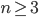
\includegraphics{images/image13.png}

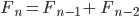
\includegraphics{images/image14.png}{~}

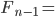
\includegraphics{images/image15.png}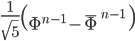
\includegraphics{images/image16.png}{~e
}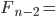
\includegraphics{images/image17.png}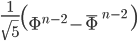
\includegraphics{images/image18.png}

{assomiglia alla forma }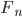
\includegraphics{images/image1.png}{~=
}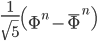
\includegraphics{images/image4.png}{~}

{ci chiediamo se }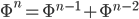
\includegraphics{images/image19.png}{~e se
}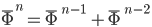
\includegraphics{images/image20.png}

{divido da entrambe le parti per
}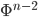
\includegraphics{images/image21.png}{~e
}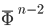
\includegraphics{images/image22.png}

{Definizione \#1}

{Utilizzeremo la notazione }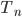
\includegraphics{images/image23.png}{~per
indicare la velocità/complessità di una particolare funzione (numero di
righe di codice eseguite) }

{Fib1 (int n) → int}

{~~~~~~~~return }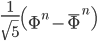
\includegraphics{images/image4.png}

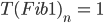
\includegraphics{images/image24.png}{~}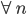
\includegraphics{images/image25.png}

{Problema: con l'aumentare di n, la funzione Fib1(n) diventa sempre più
imprecisa}

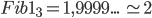
\includegraphics{images/image26.png}

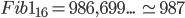
\includegraphics{images/image27.png}

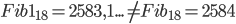
\includegraphics{images/image28.png}

{Definizione \#2}

\protect\hypertarget{t.b6ceb73d86c2dc3f3cbc86e1ad6e301e593880f5}{}{}\protect\hypertarget{t.0}{}{}

\begin{longtable}[]{@{}l@{}}
\toprule
\begin{minipage}[t]{0.97\columnwidth}\raggedright\strut
{Fib2 (}{int}{~n) → }{int}{\\
\hspace*{0.333em}\hspace*{0.333em}\hspace*{0.333em}\hspace*{0.333em}\hspace*{0.333em}\hspace*{0.333em}\hspace*{0.333em}\hspace*{0.333em}}{if}{~n
\textless{}= }{2}{~then }{return}{~}{1}{\\
\hspace*{0.333em}\hspace*{0.333em}\hspace*{0.333em}\hspace*{0.333em}\hspace*{0.333em}\hspace*{0.333em}\hspace*{0.333em}\hspace*{0.333em}}{else}{~}{return}{~Fib2(n}{-1}{)
+ Fib2(n}{-2}{)}\strut
\end{minipage}\tabularnewline
\bottomrule
\end{longtable}

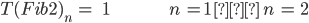
\includegraphics{images/image29.png}

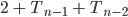
\includegraphics{images/image30.png}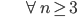
\includegraphics{images/image31.png}

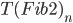
\includegraphics{images/image32.png}{~è una formula ricorsiva o ricorrenza}

\protect\hypertarget{t.b835927b516aa4a0b07c3acab4f4cd0150ff7dd8}{}{}\protect\hypertarget{t.1}{}{}

\begin{longtable}[]{@{}ll@{}}
\toprule
\begin{minipage}[t]{0.47\columnwidth}\raggedright\strut
{n}\strut
\end{minipage} & \begin{minipage}[t]{0.47\columnwidth}\raggedright\strut
$T_n$\strut
\end{minipage}\tabularnewline
\begin{minipage}[t]{0.47\columnwidth}\raggedright\strut
{1}\strut
\end{minipage} & \begin{minipage}[t]{0.47\columnwidth}\raggedright\strut
{1}\strut
\end{minipage}\tabularnewline
\begin{minipage}[t]{0.47\columnwidth}\raggedright\strut
{2}\strut
\end{minipage} & \begin{minipage}[t]{0.47\columnwidth}\raggedright\strut
{1}\strut
\end{minipage}\tabularnewline
\begin{minipage}[t]{0.47\columnwidth}\raggedright\strut
{3}\strut
\end{minipage} & \begin{minipage}[t]{0.47\columnwidth}\raggedright\strut
{2 + 1 + 1 = 4}\strut
\end{minipage}\tabularnewline
\begin{minipage}[t]{0.47\columnwidth}\raggedright\strut
{4}\strut
\end{minipage} & \begin{minipage}[t]{0.47\columnwidth}\raggedright\strut
{2 + 4 + 1 = 7}\strut
\end{minipage}\tabularnewline
\begin{minipage}[t]{0.47\columnwidth}\raggedright\strut
{5}\strut
\end{minipage} & \begin{minipage}[t]{0.47\columnwidth}\raggedright\strut
{2 + 7 + 4 = 13}\strut
\end{minipage}\tabularnewline
\bottomrule
\end{longtable}

{}

{Risolviamo la ricorrenza per determinare la complessità / bontà della
funzione esaminata.}

\begin{itemize}
\tightlist
\item
  {andamento esponenziale rispetto ad n → funzione NON efficiente}
\item
  {andamento logaritmico / proporzionale rispetto ad n → funzione
  efficiente}
\end{itemize}

\begin{center}\rule{0.5\linewidth}{\linethickness}\end{center}

\hypertarget{h.x4ciu865ga1f}{\subsubsection{\texorpdfstring{{Strumento
\#1 - albero di
ricorsione}}{Strumento \#1 - albero di ricorsione}}\label{h.x4ciu865ga1f}}

{Notiamo che }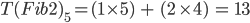
\includegraphics{images/image33.png}

{dove $(1 * 5)$ è la complessità delle foglie (5 foglie con peso 1)}

{e $(2 * 4)$ è la complessità dei nodi interni (4 nodi con peso 2)}

{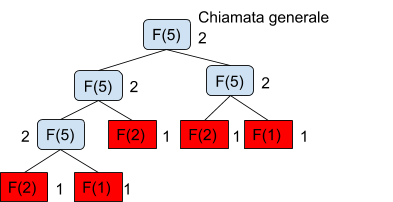
\includegraphics{images/image523.png}}

{Proprietà \#1}

{Se $T_n$ rappresenta l'albero di ricorsione relativo a $Fib2_n$, allora il numero di foglie di $T_n$ è uguale a $F_n$(con $F_n$ indichiamo l'n-esimo numero della successione di Fibonacci)}

{Dimostrazione per induzione}

{Base:}

{se n = ~1 → numero di foglie di }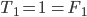
\includegraphics{images/image35.png}

{se n = ~2 → numero di foglie di }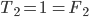
\includegraphics{images/image36.png}

{Passo induttivo:}

{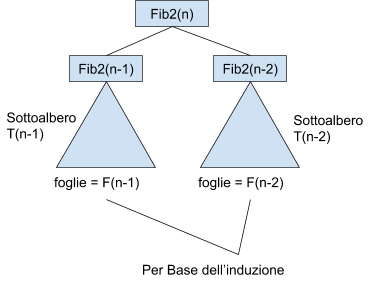
\includegraphics{images/image528.png}}

{Proprietà \#2}

{Sia $T$ un albero binario in cui ogni nodo interno ha esattamente 2 figli}

{Allora $i_T=f_T-1$, dove con $i_T$ indichiamo il numero di nodi interni dell'albero $T$ e con $f_T$ indichiamo il numero di foglie dell'albero $T$}

{Dimostrazione per induzione}

{Dimostrazione su $n$, dove $n$ è il numero di nodi di $T$}

{Base:}

$n=1${~→ OVVIO}

{Passo induttivo:}

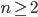
\includegraphics{images/image43.png}

{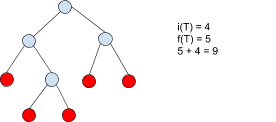
\includegraphics{images/image525.png}}

{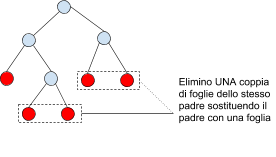
\includegraphics{images/image536.png}}

{L'albero risultante lo chiamiamo
}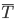
\includegraphics{images/image44.png}{~:}

{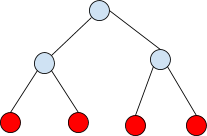
\includegraphics{images/image522.png}}

{Notiamo che }

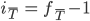
\includegraphics{images/image45.png}{*}

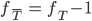
\includegraphics{images/image46.png}{**}

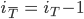
\includegraphics{images/image47.png}{~ ~}

{→ (inverto) ~ ~}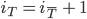
\includegraphics{images/image48.png}{~ }

{→ (sostituisco }{*}{) }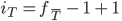
\includegraphics{images/image49.png}

{→ (semplifico) ~}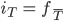
\includegraphics{images/image50.png}{~ }

{→ (sostituisco }{**}{) ~ }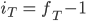
\includegraphics{images/image38.png}

{Studio complessità di }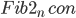
\includegraphics{images/image51.png}{l'utilizzo del metodo dell'albero di ricorsione}

{~}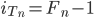
\includegraphics{images/image52.png}

{~}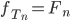
\includegraphics{images/image53.png}

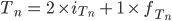
\includegraphics{images/image54.png}

{→ }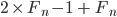
\includegraphics{images/image55.png}

{→ }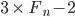
\includegraphics{images/image56.png}{~}

{Proprietà \#3}

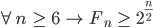
\includegraphics{images/image57.png}

{Dimostrazione per induzione}

{Base:}

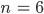
\includegraphics{images/image58.png}

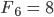
\includegraphics{images/image59.png}

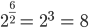
\includegraphics{images/image60.png}

{Passo induttivo:}

\includegraphics{images/image61.png}

\includegraphics{images/image62.png}

\includegraphics{images/image63.png}

\includegraphics{images/image64.png}

\includegraphics{images/image65.png}{~è sempre maggiore o uguale ad 1}

{$Fib2(n)$ risulta essere troppo poco efficiente}

\includegraphics{images/image66.png}

\includegraphics{images/image67.png}

{}

{Definiamo allora Fib3(n) utilizzando l'iterazione al posto della
ricorsione}

{}

\protect\hypertarget{t.aae11fb7a2c0b52467b2ae76a760f55e201df9fd}{}{}\protect\hypertarget{t.2}{}{}

\begin{longtable}[]{@{}l@{}}
\toprule
\begin{minipage}[t]{0.97\columnwidth}\raggedright\strut
{Fib3 (int }{n}{) --\textgreater{} int\\
\hspace*{0.333em} ~ }{//Allocazione di un array lungo n;}{\\
\hspace*{0.333em} ~ }{F}{(1) = 1; }{F}{(2) = 1;\\
\hspace*{0.333em} ~ }{For}{~i = 3 to }{n}{~\\
\hspace*{0.333em} ~ ~ ~ }{F}{(i) = }{F}{(i-1) + }{F}{(i-2);\\
\hspace*{0.333em} ~ }{Return}{~}{F}{(}{n}{)}\strut
\end{minipage}\tabularnewline
\bottomrule
\end{longtable}

{}

\includegraphics{images/image68.png}

{}

{Ci chiediamo se fib3 sia efficiente dal punto di vista della
memoria\ldots{}}

\begin{center}\rule{0.5\linewidth}{\linethickness}\end{center}

\section{\texorpdfstring{{}}{}}\label{h.t0xc4p18h6wu}

\hypertarget{h.jkxlloc1lefg}{\section{\texorpdfstring{{Notazione
asintotica: le classi O, Omega, Theta
}}{Notazione asintotica: le classi O, Omega, Theta }}\label{h.jkxlloc1lefg}}

{{[}DFI{]} 2.2; {[}CLRS{]} 3.1}

{}

{}

{}

\hypertarget{h.tn5j57miv2l8}{\section{\texorpdfstring{{Esercizi sulla
notazione asintotica. Le classi o,
omega}}{Esercizi sulla notazione asintotica. Le classi o, omega}}\label{h.tn5j57miv2l8}}

{{[}CLRS{]} 3.1}

{}

{}

\hypertarget{h.qp9ilz1tito1}{\section{\texorpdfstring{{Divide et impera.
Il teorema fondamentale delle ricorrenze (o ``Teorema master'').
Esercizi.}}{Divide et impera. Il teorema fondamentale delle ricorrenze (o Teorema master). Esercizi.}}\label{h.qp9ilz1tito1}}

{{[}DFI{]} 2.5; {[}CLRS{]} 4.3}

{}

{}

{}

\hypertarget{h.a5tr7osf4zwh}{\section{\texorpdfstring{{Rappresentazione
di una lista attraverso un vettore
(matrice)}}{Rappresentazione di una lista attraverso un vettore (matrice)}}\label{h.a5tr7osf4zwh}}

{}

{La lista è doppiamente concatenata, ovvero contiene riferimento sia
all'elemento precedente che a quello successivo.}

{}

{La costante NULL viene rappresentata da un indice che non appartiene
all'insieme degli indici del vettore (0 in pseudocodice, -1 in C)}

{}

{\includegraphics{images/image520.png}}

{}

{}

{Analogamente si può creare una lista singolarmente concatenata chiamata
FreeList contenente le celle libere (i campi Key e Previous si possono
ignorare). Essa verrà utilizzata per l'allocazione di una nuova lista.
FreeList è una variabile globale.}

{}

{All'inizio {[}\ldots{}{]} la FreeList contiene TUTTI gli oggetti non
allocati.}

{}

{Allocate\_Object()~~~~~~~~~~~~~~~~~~~~~~~~~~~~~~~~}{Complessità
}\includegraphics{images/image69.png}



\protect\hypertarget{t.6867fb3c644d0c0b07e14f5253c873dd313c05de}{}{}\protect\hypertarget{t.3}{}{}

\begin{longtable}[]{@{}l@{}}
\toprule
\begin{minipage}[t]{0.97\columnwidth}\raggedright\strut
{if}{(}{free}{~== null)\\
\hspace*{0.333em}\hspace*{0.333em}\hspace*{0.333em}\hspace*{0.333em}\hspace*{0.333em}\hspace*{0.333em}\hspace*{0.333em}\hspace*{0.333em}\hspace*{0.333em}\hspace*{0.333em}\hspace*{0.333em}\hspace*{0.333em}\hspace*{0.333em}\hspace*{0.333em}\hspace*{0.333em}\hspace*{0.333em}errore
}{``spazio esaurito''}{\\
\hspace*{0.333em}\hspace*{0.333em}\hspace*{0.333em}\hspace*{0.333em}\hspace*{0.333em}\hspace*{0.333em}\hspace*{0.333em}\hspace*{0.333em}}{else}{\\
\hspace*{0.333em}\hspace*{0.333em}\hspace*{0.333em}\hspace*{0.333em}\hspace*{0.333em}\hspace*{0.333em}\hspace*{0.333em}\hspace*{0.333em}\hspace*{0.333em}\hspace*{0.333em}\hspace*{0.333em}\hspace*{0.333em}\hspace*{0.333em}\hspace*{0.333em}\hspace*{0.333em}\hspace*{0.333em}x
= }{free}{\\
\hspace*{0.333em}\hspace*{0.333em}\hspace*{0.333em}\hspace*{0.333em}\hspace*{0.333em}\hspace*{0.333em}\hspace*{0.333em}\hspace*{0.333em}\hspace*{0.333em}\hspace*{0.333em}\hspace*{0.333em}\hspace*{0.333em}\hspace*{0.333em}\hspace*{0.333em}\hspace*{0.333em}\hspace*{0.333em}}{free}{~=
nexy{[}}{free}{{]}\\
\hspace*{0.333em}\hspace*{0.333em}\hspace*{0.333em}\hspace*{0.333em}\hspace*{0.333em}\hspace*{0.333em}\hspace*{0.333em}\hspace*{0.333em}\hspace*{0.333em}\hspace*{0.333em}\hspace*{0.333em}\hspace*{0.333em}\hspace*{0.333em}\hspace*{0.333em}\hspace*{0.333em}\hspace*{0.333em}}{return}{~x}\strut
\end{minipage}\tabularnewline
\bottomrule
\end{longtable}



{}

{\#Inserisce la cella da liberare in testa alla FreeList}

{Free\_Object(x)}{~~~~~~~~~~~~~~~~~~~~~~~~~~~~~~~~Complessità
}\includegraphics{images/image69.png}



\protect\hypertarget{t.ca6d9bfbccaf8ba905655d1fba7938b11c658c64}{}{}\protect\hypertarget{t.4}{}{}

\begin{longtable}[]{@{}l@{}}
\toprule
\begin{minipage}[t]{0.97\columnwidth}\raggedright\strut
{next{[}x{]} = }{free}{\\
\hspace*{0.333em}\hspace*{0.333em}\hspace*{0.333em}\hspace*{0.333em}\hspace*{0.333em}\hspace*{0.333em}\hspace*{0.333em}\hspace*{0.333em}}{free}{~=
x}\strut
\end{minipage}\tabularnewline
\bottomrule
\end{longtable}

{}

{}

{}

\begin{center}\rule{0.5\linewidth}{\linethickness}\end{center}

\section{\texorpdfstring{{}}{}}\label{h.eidcfonq0wug}

\hypertarget{h.rgokfftftjlb}{\section{\texorpdfstring{{Alberi}}{Alberi}}\label{h.rgokfftftjlb}}

{{[}CLRS{]} pp. 977-979}

{L'albero è un tipo particolare di grafo connesso, aciclico e non orientato.}

{Un albero radicato è una coppia $T=(N,A)$}

{$N$ è un insieme finito di nodi fra cui si distingue un nodo $R$, detto `Radice'.}

$A${~è un sottoinsieme del prodotto
cartesiano $(NxN)$,è un insieme di coppie
di nodi che chiamiamo archi.}

{In un albero, ogni nodo $v$ (eccetto la radice) ha esattamente un genitore che viene chiamato padre $u$, tale che $(u,v) \in A$}

{\includegraphics{images/image539.png}}


{Un nodo può avere 0 o più figli, un figlio è tale se esiste un arco $(u,v) \in A$}

{}

{Il numero dei figli di un nodo si chiama GRADO del nodo.}

{Un nodo senza figli è detto FOGLIA o NODO ESTERNO.}

{Un nodo non foglia è un NODO INTERNO.}

{Se due nodi hanno lo stesso padre, allora sono fratelli.}

{}

{Il cammino da}{~}$v${~ad
}\includegraphics{images/image77.png}{nell'albero
}$T${~è una sequenza di nodi
}\includegraphics{images/image78.png}{tale che soddisfa queste
condizioni:}

\includegraphics{images/image79.png}

\includegraphics{images/image80.png}

\includegraphics{images/image81.png}

{La lunghezza di un cammino è il numero di archi nel cammino oppure il
numero di nodi - 1.}

{Sia }$x${~un nodo dell'albero radicato
}$T${con radice
}\includegraphics{images/image83.png}{.}

{Qualsiasi nodo $y$ in un cammino, che parte dalla radice $r$ ed arriva ad $x$, è detto ANTENATO di $x$($x$ compreso, è antenato di se stesso).}

{Se $y$ è un antenato di $x$, allora $x$ è DISCENDENTE di $y$}

{NB: Ogni nodo è DISCENDENTE ed ANTENATO di sè stesso.}

{Se $y$ è un antenato di $x$ ed $x$ è diverso da $y$, allora $y$ è un ANTENATO PROPRIO di $x$ ed $x$ è DISCENDENTE PROPRIO di $y$.}

{Il sottoalbero con radice in $x$ è l'albero indotto dai discendenti di $x$}

{La profondità di un nodo $x$ è la lunghezza del cammino dalla radice ad $x$.}

{Un livello di un albero è costituito da tutti i nodi che stanno alla stessa profondità. }

{L'altezza di un nodo $x$ è la lunghezza del più lungo cammino che scende da $x$ alle foglie (qualsiasi foglia) di profondità massima.}

{L'altezza di un albero è l'altezza del nodo radice.}

{L'altezza è la massima profondità di un qualsiasi nodo dell'albero.}

\hypertarget{h.rmzlh8kpnju}{\subsection{\texorpdfstring{{Alberi binari
(Albero k-ario con K =
2)}}{Alberi binari (Albero k-ario con K = 2)}}\label{h.rmzlh8kpnju}}

{Gli alberi binari sono definiti in modo ricorsivo:}

\begin{itemize}
\tightlist
\item
  {Un albero vuoto è binario}
\item
  {Un albero costituito da un nodo (radice) ,}
\end{itemize}

{~~~~~~~~~~~~~~~~da un albero binario detto sottoalbero sinistro della
radice,}

{~~~~~~~~~~~~~~~~e da un'altro albero binario detto sottoalbero destro
della radice}

{~~~~~~~~~~~~~~~~è detto un albero binario.}

{}

\hypertarget{h.chua2o837in5}{\subsection{\texorpdfstring{{Albero
k-ario}}{Albero k-ario}}\label{h.chua2o837in5}}

{E' un albero in cui i figli si un nodo sono etichettati con interi
positivi distinti e le etichette maggiori di
}$K${~sono assenti = ogni nodo può
avere al più }$K${~figli.}

{}

{Un albero K-ario completo è tale quando tutte le foglie hanno la stessa
profondità e tutti i nodi interni hanno grado
}$K${~}

{}

{ALGORITMO}

{Trovare l'algoritmo per determinare la completezza di un albero}

{Dimostro per induzione che le foglie sono $K^h$}


{$h=0$ (caso base): $K^0=1$, OK}

{Assumiamo che per un albero di altezza $h$ sia vero che $n=K^h$}

{Lo dimostro per $h+1$}

{Il numero di nodi di profondità $h$ è $K^h$ per ipotesi}

{Il numero di nodi di profondità $h+1$ è $K^h*K=K^{h+1}$, OK}

{ALGORITMO}

{Trovare il numero di foglie e il numero di nodi interni di un albero k-ario completo di altezza $h$}

\includegraphics{images/image93.png}{~è una sommatoria GEOMETRICA, si
semplifica in }\includegraphics{images/image94.png}{, quindi
}\includegraphics{images/image95.png}

{Altezza di un albero k-ario completo con $n$ nodi:}

\includegraphics{images/image96.png}{~→
}\includegraphics{images/image97.png}{~→
}\includegraphics{images/image98.png}

{Proprietà}

{Dimostrare per induzione che in un albero BINARIO completo non nullo avente $n$ nodi, il numero di foglie è $\frac{n+1}{2}$}

\hypertarget{h.8kg49eb4dpz1}{\subsubsection{\texorpdfstring{{Tipo di dato ALBERO}}{Tipo di dato ALBERO}}\label{h.8kg49eb4dpz1}}


{Struttura:}

{Insieme di nodi}

{Insieme di archi}


{Le operazioni del tipo ALBERO:}


{~~~~~~~~newTree() → T~~~~~~~~~~~~~~~~Nuovo albero T}

{~~~~~~~~numNodi(T) → int~~~~~~~~~~~~~~~~Numero di nodi presenti in T}

{~~~~~~~~grado(T,N) → int~~~~~~~~~~~~~~~~Numero di figli di N, N
appartenente a T}

{~~~~~~~~padre(T,N) → int~~~~~~~~~~~~~~~~Nodo padre, null se N è radice,
~N appartenente a T}

{~~~~~~~~figli(T,N) → int{[}{]}~~~~~~~~~~~~~~~~Lista contenente i figli
del nodo N, N appartenente a T}

{}

\hypertarget{h.ueuovjwdu9zj}{\section{\texorpdfstring{{Rappresentazione
di alberi tramite
array}}{Rappresentazione di alberi tramite array}}\label{h.ueuovjwdu9zj}}

{}

\subsection{Utilizzo del vettore padri}

{Sia $T=(N,A), N = \{n_1,n_2,...,n_n\}$}

{Costruisco un vettore di dimensione $n$, le cui celle contengono copie di $(i,u)$. Con $i$ indichiamo l'informazione del nodo e con $u$ indichiamo il nodo padre (indice).}

$\forall v \in [1,n]$

{p{[}v{]} → info = contenuto}

{p{[}v{]} → padre = indice del padre,$(u,v) \in A(archi)$, se $v$ è radice il padre è NULL/-1/0}

{Spazio per memorizzare $n=\Theta(n)$}

\subsubsection{Implementazioni}

{Padre - Complessità $\Theta(1)$}

\lstinputlisting{code/tree_vecp_padre.txt}

{Figli - Complessità $\Theta(n)$}

\lstinputlisting{code/tree_vecp_figli.txt}

\subsection{Utilizzo del vettore posizionale}

{L'albero deve essere completo e con $k \geq 2$. La ricerca è ottimizzata rispetto all'albero dei padri. Ogni nodo ha una posizione prestabilita.}

{Utilizzo un vettore posizionale $P$ di dimensione $n$ tale che }

\begin{enumerate}
\tightlist
\item
  {0 è la posizione della radice}
\item
  {l'i-esimo figlio di un certo nodo v è in posizione
  }\includegraphics{images/image110.png}{, con
  }\includegraphics{images/image111.png}
\end{enumerate}

{un nodo $f$ è foglia se non ha figli, quindi se }\includegraphics{images/image113.png}

{Il padre del nodo $f$ è in posizione $\floor{\frac{f-1}{k}}$ (parte intera inferiore) e i figli si trovano tra $kv+1$ e $kv+1+i-1$.

\subsubsection{Implementazioni}

{Padre - Complessità $\Theta(1)$}

\lstinputlisting{code/tree_vec_padre.txt}

{Figli - Complessità $\Theta(k)$, con $k$ = grado di $v$}

\lstinputlisting{code/tree_vec_figli.txt}

\subsection{Utilizzo di strutture collegate}

\paragraph{Parent + Childs}

{}

{Ogni nodo è un record con i seguenti campi:}

{~~~~~~~~k : informazione}

{~~~~~~~~p : puntatore al padre}



{~~~~~~~~Se il numero di figli è noto}

{}

{~~~~~~~~~~~~~~~~left : puntatore al figlio sinistro}

{~~~~~~~~~~~~~~~~right : puntatore al figlio destro}

{}

{Altrimenti si utilizza una lista di puntatori ai propri figli}

{c {[}{]} : lista di puntatori ai figli~~~~~~~~}

{Se ogni nodo ha grado al più $k$, è possibile mantenere in ogni nodo un puntatore a ciascuno dei possibili $k$ figli}

{Spazio necessario: $\Theta(nk)$, se $k$ costante allora $\Theta(n)$}

\subsubsection{Implementazioni:}

{Padre - Complessità $O(1)$}

\lstinputlisting{code/tree_pc_padre.txt}

{Figli - Complessità $O(k)$, con $k$ = grado di $v$ }

{Con $k$ non noto si utilizza un ciclo che scorre c{[}{]}}

\lstinputlisting{code/tree_pc_figli.txt}

\paragraph{Parent + Left child + Right sibling}

{Ogni nodo è un record con i seguenti campi:}

{~~~~~~~~k : informazione}

{~~~~~~~~p : puntatore al padre}

{~~~~~~~~left\_child : puntatore al figlio sinistro}

{~~~~~~~~right\_sibling : puntatore al fratello immediatamente a destra}

\subsubsection{Implementazioni}

{Padre - Complessità $\Theta(1)$}

\lstinputlisting{code/tree_plcrs_padre.txt}

{Figli - Complessità $\Theta(k)$ con $k$ = grado di $v$}

\lstinputlisting{code/tree_plcrs_figli.txt}

\section{Algoritmi di visita degli Alberi}

{{[}DFI{]} pp. 77-80}

\subsubsection{Visita generica}

\lstinputlisting{code/visita_generica.txt}

{Dimostrare che ha costo LINEARE}\textsuperscript{\protect\hyperlink{cmnt2}{{[}b{]}}}

\hypertarget{h.6xasx7f8zgn1}{\paragraph{\texorpdfstring{{Teorema}}{Teorema}}\label{h.6xasx7f8zgn1}}

{L'algoritmo di visita, applicato alla radice di un albero con $m$ nodi, termina in $O(m)$ iterazioni. Lo spazio usato è $O(n)$}

\hypertarget{h.zdc8liauzt1c}{\paragraph{\texorpdfstring{{Dimostrazione}}{Dimostrazione}}\label{h.zdc8liauzt1c}}

{Hp: L'inserimento e la cancellazione da $S$ sono effettuati in tempo costante}

{Ogni nodo verrà inserito ed estratto dall'insieme $s$ una sola volta, perchè in un albero non si può tornare ad un nodo a partire dai suoi figli.}

{Quindi le iterazioni del ciclo while saranno al più $O(n)$}

{Poiché ogno nodo compare al più una volta in $S$, lo spazio richiesto non è più alto di $O(n)$}

\subsubsection{Visita DFS - Depth first search - Ricerca in profondità}

{Seguiamo tutti i figli sinistri, andando in profondità fino a che non si raggiunge la prima foglia sinistra. Solo quando il sottoalbero sx è stato completamente visitato, si passa ~a visitare il sottoalbero dx}

\lstinputlisting{code/dfs_visit.txt}

\subsubsection{Visita BFS - Breadth first search - Ricerca in ampiezza}

\section{Heap}

{Heap: albero quasi completo con tutti i nodi dell'ultimo livello a sinistra}

{MaxHeap: La radice ha valore maggiore o uguale a quello dei figli}

{MinHeap: La radice ha valore minore o uguale a quello dei figli}

\subsubsection{Lemma 2}

{Nell'array che rappresenta un heap di $n$ elementi, le foglie sono i nodi con indici che vanno alle posizioni}

$\frac{n}{2}+1,\frac{n}{2}+2,...,n$

\includegraphics{images/image526.png}

{Elemento}

{16}

{15}

{10}

{14}

{7}

{9}

{3}

{2}

{8}

{1}

{Posizione}

{1°}

{2°}

{3°}

{4°}

{5°}

{6°}

{7°}

{8°}

{9°}

{10°}

{}

{}

{}

{}

\includegraphics{images/image124.png}

\includegraphics{images/image125.png}

\includegraphics{images/image126.png}

\includegraphics{images/image127.png}

\includegraphics{images/image128.png}

{n}

\hypertarget{h.wlc8yrs7inpk}{\subsubsection{\texorpdfstring{{Lemma 3:}}{Lemma 3:}}\label{h.wlc8yrs7inpk}}

{Il teorema definisce la numerosità di nodi con una certa altezza:}

{Ci sono al massimo $\frac{n}{2^{h+1}}$ nodi di altezza}\textsuperscript{\protect\hyperlink{cmnt3}{{[}c{]}}}{~}{h}{~in
un qualsiasi heap di $n$ elementi}

\hypertarget{h.t1rcecigqmbx}{\subsubsection{\texorpdfstring{{Max\_heapify}}{Max\_heapify}}\label{h.t1rcecigqmbx}}

{L'operazione max\_heapify permette di mantenere le proprietà di maxheap}

{Precondizioni:}

{Gli alberi binari con radice in left(i) e right(i) sono maxheap}

{Postcondizioni:}

{~~~~~~~~L'albero radicato in $i$ è un maxheap}

\lstinputlisting{code/max_heapify.txt}

{Tempo di esecuzione : $O(h)$ dove $h$ è l'altezza del nodi i poichè l'heap ha altezza $log(n)$ (LEMMA 2)}

\hypertarget{h.symae1e4ut5b}{\subsection{\texorpdfstring{{Dato un vettore disordinato, costruire un heap}}{Dato un vettore disordinato, costruire un heap}}\label{h.symae1e4ut5b}}

\lstinputlisting{code/build_maxheap.txt}

{Invariante: ogni nodo in posizione \includegraphics{images/image130.png} è radice di un maxheap, con n = }

{Sembrerebbe complessa }\includegraphics{images/image131.png}{ma max\_heapify lavora principalmente su foglie, }{quindi la complessità è lineare }\includegraphics{images/image132.png}{.}

\includegraphics{images/image133.png}

{L'ultima sommatoria è la serie nota}\includegraphics{images/image134.png}

{Con }\includegraphics{images/image135.png}{,}\includegraphics{images/image136.png}

{Quindi }\includegraphics{images/image137.png}

\subsection{Heapsort}

\lstinputlisting{code/heapsort.txt}

{INV = Il sottoarray che va dalla posizione $1$ alla posizione $i$ è un maxheap che contiene gli elementi più piccoli del intero vettore di partenza, mentre }\includegraphics{images/image138.png}{contiene gli $n-1$ elementi più grandi di $A[1..n]$ ordinati}{.}

\hypertarget{h.rdu8s741ww8w}{\subsubsection{\texorpdfstring{{Teorema}}{Teorema}}\label{h.rdu8s741ww8w}}

{L'algoritmo HeapSort ordina in loco $n$ elementi eseguendo nel peggiore dei casi $O(nlog(n))$ confronti in quanto algoritmo basato sui confronti.}

\hypertarget{h.jih9riph7gns}{\subsection{\texorpdfstring{{Code di
priorità}}{Code di priorità}}\label{h.jih9riph7gns}}

{{[}CLRS{]} pp. 135-140}

{Struttura dati che serve a mantenere un insieme dinamico i cui elementi ( aggiungibili e rimovibili ) hanno un valore associato detto chiave o peso.}

{Esistono due tipi di code di priorità:}

\begin{itemize}
\tightlist
\item
  {MaxPriorità (Si utilizza la struttura MaxHeap)}
\item
  {MinPriorità (Si utilizza la struttura MinHeap)}
\end{itemize}

{Le operazioni delle code di priorità massima/minima sono:}

{Insert( Coda s , Elemento X) : Inserisce l'elemento $X$ in $S$}

{Maximum( Coda s ): Restituisce l'elemento di $S$ con la chiave maggiore senza rimuoverlo}

{Minimum( Coda s) : Restituisce l'elemento di $S$ con la chiave minore senza rimuoverlo}

{Extract\_max( Coda s) : Elimina e restituisce l'elemento di $S$ con la chiave maggiore}

{Extract\_min( Coda s) : Elimina e restituisce l'elemento di $S$ con la chiave minore}

{Increase\_key( Coda s, Elemento x, Chiave k) : Incrementa il valore della chiave di $X$ al nuovo valore $K$. Si suppone che $K$ sia maggiore o uguale al valore corrente della chiave di $X$, $K \geq chiave(X)$}

{Decrease\_key( Coda s, Elemento x, Chiave k) : Decrementa il valore della chiave di $X$ al nuovo valore $K$. Si suppone che $K$ sia minore o uguale al valore corrente della chiave di $X$, $K \leq chiave(X)$}

\begin{center}\rule{0.5\linewidth}{\linethickness}\end{center}

\subsection{Implementazione di code di massima priorità con le strutture Heap}}

\begin{longtable}[]{@{}l@{}}
\toprule
\begin{minipage}[t]{0.97\columnwidth}\raggedright\strut
{Heap\_maximum(Heap A)\\
\hspace*{0.333em}\hspace*{0.333em}\hspace*{0.333em}\hspace*{0.333em}\hspace*{0.333em}\hspace*{0.333em}\hspace*{0.333em}\hspace*{0.333em}}{if}{~(
A.heapSize \textless{} }{1}{~)\\
\hspace*{0.333em}\hspace*{0.333em}\hspace*{0.333em}\hspace*{0.333em}\hspace*{0.333em}\hspace*{0.333em}\hspace*{0.333em}\hspace*{0.333em}\hspace*{0.333em}\hspace*{0.333em}\hspace*{0.333em}\hspace*{0.333em}\hspace*{0.333em}\hspace*{0.333em}\hspace*{0.333em}\hspace*{0.333em}}{error}{~}{``heap
underflow''}{\\
\hspace*{0.333em}\hspace*{0.333em}\hspace*{0.333em}\hspace*{0.333em}\hspace*{0.333em}\hspace*{0.333em}\hspace*{0.333em}\hspace*{0.333em}}{else}{\\
\hspace*{0.333em}\hspace*{0.333em}\hspace*{0.333em}\hspace*{0.333em}\hspace*{0.333em}\hspace*{0.333em}\hspace*{0.333em}\hspace*{0.333em}\hspace*{0.333em}\hspace*{0.333em}\hspace*{0.333em}\hspace*{0.333em}\hspace*{0.333em}\hspace*{0.333em}\hspace*{0.333em}\hspace*{0.333em}}{max}{~=
A{[}}{1}{{]}\\
\hspace*{0.333em}\hspace*{0.333em}\hspace*{0.333em}\hspace*{0.333em}\hspace*{0.333em}\hspace*{0.333em}\hspace*{0.333em}\hspace*{0.333em}\hspace*{0.333em}\hspace*{0.333em}\hspace*{0.333em}\hspace*{0.333em}\hspace*{0.333em}\hspace*{0.333em}\hspace*{0.333em}\hspace*{0.333em}}{return}{~}{max}\strut
\end{minipage}\tabularnewline
\bottomrule
\end{longtable}

{Complessità di Heap Maximum : $O(1)$}

\begin{longtable}[]{@{}l@{}}
\toprule
\begin{minipage}[t]{0.97\columnwidth}\raggedright\strut
{Heap\_extract\_max(Heap A)\\
\hspace*{0.333em}\hspace*{0.333em}\hspace*{0.333em}\hspace*{0.333em}\hspace*{0.333em}\hspace*{0.333em}\hspace*{0.333em}\hspace*{0.333em}}{if}{~(
A.heapSize \textless{} }{1}{~)\\
\hspace*{0.333em}\hspace*{0.333em}\hspace*{0.333em}\hspace*{0.333em}\hspace*{0.333em}\hspace*{0.333em}\hspace*{0.333em}\hspace*{0.333em}\hspace*{0.333em}\hspace*{0.333em}\hspace*{0.333em}\hspace*{0.333em}\hspace*{0.333em}\hspace*{0.333em}\hspace*{0.333em}\hspace*{0.333em}}{error}{~}{``heap
underflow''}{\\
\hspace*{0.333em}\hspace*{0.333em}\hspace*{0.333em}\hspace*{0.333em}\hspace*{0.333em}\hspace*{0.333em}\hspace*{0.333em}\hspace*{0.333em}}{else}{\\
\hspace*{0.333em}\hspace*{0.333em}\hspace*{0.333em}\hspace*{0.333em}\hspace*{0.333em}\hspace*{0.333em}\hspace*{0.333em}\hspace*{0.333em}\hspace*{0.333em}\hspace*{0.333em}\hspace*{0.333em}\hspace*{0.333em}\hspace*{0.333em}\hspace*{0.333em}\hspace*{0.333em}\hspace*{0.333em}}{max}{~=
A{[}}{1}{{]}\\
\hspace*{0.333em}\hspace*{0.333em}\hspace*{0.333em}\hspace*{0.333em}\hspace*{0.333em}\hspace*{0.333em}\hspace*{0.333em}\hspace*{0.333em}\hspace*{0.333em}\hspace*{0.333em}\hspace*{0.333em}\hspace*{0.333em}\hspace*{0.333em}\hspace*{0.333em}\hspace*{0.333em}\hspace*{0.333em}A{[}}{1}{{]}
= A{[} A.heapSize {]}\\
\hspace*{0.333em}\hspace*{0.333em}\hspace*{0.333em}\hspace*{0.333em}\hspace*{0.333em}\hspace*{0.333em}\hspace*{0.333em}\hspace*{0.333em}\hspace*{0.333em}\hspace*{0.333em}\hspace*{0.333em}\hspace*{0.333em}\hspace*{0.333em}\hspace*{0.333em}\hspace*{0.333em}\hspace*{0.333em}A.heapSize
-= }{1}{\\
\hspace*{0.333em}\hspace*{0.333em}\hspace*{0.333em}\hspace*{0.333em}\hspace*{0.333em}\hspace*{0.333em}\hspace*{0.333em}\hspace*{0.333em}\hspace*{0.333em}\hspace*{0.333em}\hspace*{0.333em}\hspace*{0.333em}\hspace*{0.333em}\hspace*{0.333em}\hspace*{0.333em}\hspace*{0.333em}}{max\_heapify}\textsuperscript{\protect\hyperlink{cmnt6}{{[}f{]}}}{~(
A , }{1}\textsuperscript{\protect\hyperlink{cmnt7}{{[}g{]}}}{~)\\
\hspace*{0.333em} ~ ~ ~ ~ ~}{return}{~}{max}\strut
\end{minipage}\tabularnewline
\bottomrule
\end{longtable}

{Complessità di Heap Extract Max :}$O(log(n))$

{}

{}

{}

\protect\hypertarget{t.0e5b1be2be4b16559db247c1c6d503c6b86fb0d1}{}{}\protect\hypertarget{t.21}{}{}

\begin{longtable}[]{@{}l@{}}
\toprule
\begin{minipage}[t]{0.97\columnwidth}\raggedright\strut
{Heap\_Increase\_Key(Heap A, Nodo i, Key K)\\
\hspace*{0.333em}\hspace*{0.333em}\hspace*{0.333em}\hspace*{0.333em}\hspace*{0.333em}\hspace*{0.333em}\hspace*{0.333em}\hspace*{0.333em}}{if}{~(
K \textless{} A{[}i{]} )\\
\hspace*{0.333em}\hspace*{0.333em}\hspace*{0.333em}\hspace*{0.333em}\hspace*{0.333em}\hspace*{0.333em}\hspace*{0.333em}\hspace*{0.333em}\hspace*{0.333em}\hspace*{0.333em}\hspace*{0.333em}\hspace*{0.333em}\hspace*{0.333em}\hspace*{0.333em}\hspace*{0.333em}\hspace*{0.333em}error
}{``la nuova chiave è più piccola di quella esistente''}{\\
\hspace*{0.333em}\hspace*{0.333em}\hspace*{0.333em}\hspace*{0.333em}\hspace*{0.333em}\hspace*{0.333em}\hspace*{0.333em}\hspace*{0.333em}}{else}{\\
\hspace*{0.333em}\hspace*{0.333em}\hspace*{0.333em}\hspace*{0.333em}\hspace*{0.333em}\hspace*{0.333em}\hspace*{0.333em}\hspace*{0.333em}\hspace*{0.333em}\hspace*{0.333em}\hspace*{0.333em}\hspace*{0.333em}\hspace*{0.333em}\hspace*{0.333em}\hspace*{0.333em}\hspace*{0.333em}A{[}i{]}
= K\\
\hspace*{0.333em}\hspace*{0.333em}\hspace*{0.333em}\hspace*{0.333em}\hspace*{0.333em}\hspace*{0.333em}\hspace*{0.333em}\hspace*{0.333em}\hspace*{0.333em}\hspace*{0.333em}\hspace*{0.333em}\hspace*{0.333em}\hspace*{0.333em}\hspace*{0.333em}\hspace*{0.333em}\hspace*{0.333em}}{while}\textsuperscript{\protect\hyperlink{cmnt8}{{[}h{]}}\protect\hyperlink{cmnt9}{{[}i{]}}}{~(
i \textgreater{} }{1}{~}{AND}{~A{[}i{]} \textgreater{}
A{[}}{parent}{(i){]} )\\
\hspace*{0.333em}\hspace*{0.333em}\hspace*{0.333em}\hspace*{0.333em}\hspace*{0.333em}\hspace*{0.333em}\hspace*{0.333em}\hspace*{0.333em}\hspace*{0.333em}\hspace*{0.333em}\hspace*{0.333em}\hspace*{0.333em}\hspace*{0.333em}\hspace*{0.333em}\hspace*{0.333em}\hspace*{0.333em}\hspace*{0.333em}\hspace*{0.333em}\hspace*{0.333em}\hspace*{0.333em}\hspace*{0.333em}\hspace*{0.333em}\hspace*{0.333em}\hspace*{0.333em}scambia
( A{[}i{]} , A{[}}{parent}{(i){]} )\\
\hspace*{0.333em}\hspace*{0.333em}\hspace*{0.333em}\hspace*{0.333em}\hspace*{0.333em}\hspace*{0.333em}\hspace*{0.333em}\hspace*{0.333em}\hspace*{0.333em}\hspace*{0.333em}\hspace*{0.333em}\hspace*{0.333em}\hspace*{0.333em}\hspace*{0.333em}\hspace*{0.333em}\hspace*{0.333em}\hspace*{0.333em}\hspace*{0.333em}\hspace*{0.333em}\hspace*{0.333em}\hspace*{0.333em}\hspace*{0.333em}\hspace*{0.333em}\hspace*{0.333em}i
= }{parent}{(i)}\strut
\end{minipage}\tabularnewline
\bottomrule
\end{longtable}

{Complessità di Heap Increase Key : $O(log(n))$}


{Invariante del while:
L'array $A[i,...,A.heapSize]$ soddisfa le proprietà di maxHeap tranne una possibile violazione: A{[}i{]} potrebbe essere più grande di A{[}parent(i){]}}

{Con un Heap di n elementi, la complessità è $O(log(n))$ in quanto il cammino dal nodo fino alla radice ha lunghezza }$O(log(n))$

\lstinputlisting{code/heap_insert.txt}

{Complessità di Heap\_Insert : }$O(log(n))$

{La ricerca su una cosa di priorità, nel caso peggiore, ha costo }$O(n)$

{Premessa : $1 \leq i \leq A.heapSize$}

\lstinputlisting{code/heap_delete.txt}

{Complessità di Heap Delete : }$O(log(n))$

\hypertarget{h.r8bopy9q4g8f}{\subsubsection{\texorpdfstring{{Esercizi}}{Esercizi}}\label{h.r8bopy9q4g8f}}

{Esercizio 1 }{: }

{Scrivere una funzione che determini se un albero è quasi completo. Gli output devono essere 1 se l'albero è quasi completo o 0 se non lo è. }{L'albero è rappresentato con notazione left e right.}

{Note: notiamo che non è sufficiente sapere se un albero è quasi completo o meno, necessitiamo anche di un valore per rappresentare l'albero completo.}

{Gli output saranno quindi: 0 - albero completo, 1 - albero quasi completo, 2 - albero non quasi completo.}


\lstinputlisting{code/is_quasi_completo.txt}

\lstinputlisting{code/is_quasi_completo_aux.txt}

{Complessità di is\_quasi\_completo : $O(n)$}

\includegraphics{images/image148.png}

{Esercizio 2 : }

{Siano dati due alberi binari completi di radice $r$ ed $s$ aventi la stessa altezza $h$ e dimensione totale ( somma dei nodi dei due alberi ) $n$. Le chiavi memorizzate nei nodi soddisfano la proprietà di maxheap. Si vuole creare un unico albero quasi completo maxheap, fusione dei due alberi, con altezza $h+1$ e dimensione $n$.}

{Le seguenti soluzioni vengono accettate:}

\begin{enumerate}
\tightlist
\item
  {Soluzione di costo e tempo }\includegraphics{images/image149.png}{~e in spazio aggiuntivo }\includegraphics{images/image149.png}
\item
  {Soluzione (più elegante) di costo e tempo $O(log(n))$ e spazio aggiuntivo costante}
\end{enumerate}

{Soluzione :}

\begin{enumerate}
\tightlist
\item
  {Soluzione di costo e tempo }\includegraphics{images/image149.png}{~e in spazio aggiuntivo }\includegraphics{images/image149.png}
\end{enumerate}

{}

{~~~~~~~~~~~~~~~~~~~~~~~~Vettore di n elementi v. (spazio aggiuntivo
}\includegraphics{images/image149.png}{)}

{~~~~~~~~~~~~~~~~~~~~~~~~Carichiamo il vettore con i valori di r ed s.
}\includegraphics{images/image149.png}

{~~~~~~~~~~~~~~~~~~~~~~~~Applichiamo build\_maxheap all'intero vettore
v.}\includegraphics{images/image149.png}

{~~~~~~~~~~~~~~~~~~~~~~~~Creo l'albero corrispondente.
}\includegraphics{images/image149.png}

{}

\begin{enumerate}
\setcounter{enumi}{1}
\tightlist
\item
  {Soluzione di costo e tempo $O(log(n))$ e spazio aggiuntivo costante}
\end{enumerate}

{Non possiamo fare altro che modificare le strutture a nostra disposizione, non usiamo strutture ausiliarie.}

{}

{Prendo come radice il nodo foglia x più a destra dell'albero s.
~}\includegraphics{images/image150.png}

{Assegno x.left ad s e x.right as r.}

{Applico la max\_heapify al nuovo nodo radice x.
}\includegraphics{images/image150.png}

\begin{center}\rule{0.5\linewidth}{\linethickness}\end{center}

{}

\hypertarget{h.7gslm72cwwxs}{\section{\texorpdfstring{{Limite inferiore
per l'ordinamento per
confronti}}{Limite inferiore per l'ordinamento per confronti}}\label{h.7gslm72cwwxs}}

{{[}CLRS{]} pp. 157-159}

{}

{Fino ad ora abbiamo visto i seguenti algoritmi di ordinamento, tutti basati sul confronto.}

{}

\protect\hypertarget{t.d27200ce3c3d6e65597fb549126b470657d85de0}{}{}\protect\hypertarget{t.26}{}{}

\begin{longtable}[]{@{}ll@{}}
\toprule
\begin{minipage}[t]{0.47\columnwidth}\raggedright\strut
{MergeSort}\strut
\end{minipage} & \begin{minipage}[t]{0.47\columnwidth}\raggedright\strut
\includegraphics{images/image151.png}\strut
\end{minipage}\tabularnewline
\begin{minipage}[t]{0.47\columnwidth}\raggedright\strut
{QuickSort}\strut
\end{minipage} & \begin{minipage}[t]{0.47\columnwidth}\raggedright\strut
{Caso medio : }\includegraphics{images/image151.png}{, caso pessimo :
}\includegraphics{images/image152.png}\strut
\end{minipage}\tabularnewline
\begin{minipage}[t]{0.47\columnwidth}\raggedright\strut
{HeapSort}\strut
\end{minipage} & \begin{minipage}[t]{0.47\columnwidth}\raggedright\strut
\includegraphics{images/image151.png}\strut
\end{minipage}\tabularnewline
\begin{minipage}[t]{0.47\columnwidth}\raggedright\strut
{InsertionSort}\strut
\end{minipage} & \begin{minipage}[t]{0.47\columnwidth}\raggedright\strut
\includegraphics{images/image152.png}\strut
\end{minipage}\tabularnewline
\bottomrule
\end{longtable}

{}

{}

{Ci domandiamo, }{è possibile infrangere il limite inferiore di }\includegraphics{images/image151.png}{? Dimostreremo che NON è possibile farlo con algoritmi basati sul confronto.}

{}

{Analizziamo il limite inferiore degli algoritmi basati sul confronto:}

\includegraphics{images/image149.png}{è il limite banale, in quanto devo analizzare n elementi. Questo limite è tuttavia irrealistico e insensato.}

{}

{Tutti gli algoritmi basati sul confronto hanno come limite inferiore
}\includegraphics{images/image153.png}{. Per dimostrarlo facciamo uso
degli }{alberi di decisione.}

{}

{Un albero di decisione è un'astrazione di un qualsiasi algoritmo di ordinamento basato sui confronti.}

\hypertarget{h.oynrnvh2y1cp}{\subsection{\texorpdfstring{{Esempio:
Ordina 3 elementi}}{Esempio: Ordina 3 elementi}}\label{h.oynrnvh2y1cp}}

{}

{\includegraphics{images/image531.png}}

Esempio: $<6,8,3>$

\begin{tikzpicture}[->,>=stealth',level/.style={sibling distance = 5cm/#1, level distance = 1.5cm}] 
\node [arn_n] {1:2}
    child{ node [arn_r] {2:3} 
            child{ node [arn_n] {10} 
            	child{ node [arn_r] {5} edge from parent node[above left]
                         {$x$}} %for a named pointer
							child{ node [arn_x] {}}
            }
            child{ node [arn_n] {1:3}
							child{ node [arn_r] {18}}
							child{ node [arn_x] {}}
            }                            
    }
    child{ node [arn_r] {1:3}
            child{ node [arn_n] {38} 
							child{ node [arn_r] {36}}
							child{ node [arn_r] {39}}
            }
            child{ node [arn_n] {2:3}
							child{ node [arn_r] {49}}
							child{ node [arn_x] {}}
            }
		}
; 
\end{tikzpicture}

{Questa struttura assomiglia
all'InsertionSort}\textsuperscript{\protect\hyperlink{cmnt15}{{[}o{]}}}

{}

{Per un input $A = <A_1,...,A_n>$ di dimensione $n$, ogni nodo interno è etichettato da una coppia $i:j$ dove $i,j$ sono indici dell'insieme da ordinare.}

\begin{itemize}
\tightlist
\item
  {$i:j$ significa confrontare $A_i$ con $A_j$}
\item
  {il sottoalbero sinistro dà i successivi confronti se $A_i \leq A_j$}
\item
  {il sottoalbero destro dà i successivi confronti se $A_i > A_j$}
\item
  {ogni foglia fornisce una permutazione dell'input tale che se io vado a prendere gli elementi dell'input, ordinati a seconda della permutazione, ottengo l'insieme ordinato in ordine crescente}
\end{itemize}

{Dato un qualsiasi algoritmo di ordinamento basato sul confronto, è
possibile costruirmi gli alberi di decisione.}

\begin{itemize}
\tightlist
\item
  {Ogni valore di n è associato ad un proprio albero di decisione.}
\item
  {L'albero modella tutte le tracce possibile di esecuzione.}
\item
  {Il tempo di esecuzione (cioè il numero di confronti necessari) è la
  lunghezza di un cammino sull'albero.}
\item
  {Il tempo di esecuzione nel caso peggiore è il più lungo cammino
  dell'albero, }{ovvero l'altezza dell'albero.}
\end{itemize}

{Mi basta quindi trovare la dimensione dell'albero di decisione per
determinare il tempo di esecuzione.}

\hypertarget{h.prflgx3s7s1g}{\subsection{\texorpdfstring{{Quanto è grande un albero di decisione?}}{Quanto è grande un albero di decisione?}}\label{h.prflgx3s7s1g}}

\hypertarget{h.cphw2k3mqktf}{\subsubsection{\texorpdfstring{{Quante foglie contiene?}}{Quante foglie contiene?}}\label{h.cphw2k3mqktf}}

{L'albero ha come minimo $n!$ foglie poichè, per essere corretto, ogni permutazione deve comparire almeno una volta.}

\hypertarget{h.yiy1tipj4aof}{\paragraph{\texorpdfstring{{Lemma 2:}}{Lemma 2:}}\label{h.yiy1tipj4aof}}

{Un albero binario di altezza h ha al più $2^h$ foglie.}

{Dimostrazione per induzione:}

\begin{itemize}
\tightlist
\item
  {Se $h=0$ abbiamo un albero costituito da un solo nodo radice che è l'unica foglia. Ovviamente con $h=0$, $1 \leq 2^h$ è verificata, infatti $1\leq 2^0$.}
\item
  {Assumiamo vera la proprietà per alberi binari di altezza $k<h$ e lo dimostro per $h$. Sia $r$ la radice dell'albero $t$. }
\end{itemize}

\begin{itemize}
\tightlist
\item
  {Se $t$ ha un solo figlio allora il numero di foglie di $t$ è uguale a quello del figlio che ha altezza $h-1$. }{Per ipotesi induttiva}{: Il numero delle foglie del sottoalbero figlio è minore di $2^{h-1}$, che è minore di $2^h$.}
\item
  {Se sono presenti entrambi il figlio sx e il figlio dx, allora il numero delle foglie è dato dalla somma delle foglie dei due sottoalberi. Siano $h_L,h_R$ le altezze
  dei due figli. Entrambe sono minori di $h$.}
\end{itemize}

\includegraphics{images/image169.png}

\includegraphics{images/image170.png}{ma
}\includegraphics{images/image171.png}{, quindi
}$f \leq 2^h$

{Quindi il numero delle foglie è compreso tra $n!$ e $2^h$.}



\hypertarget{h.hr66c3ikhdcj}{\paragraph{\texorpdfstring{{Teorema:}}{Teorema:}}\label{h.hr66c3ikhdcj}}

{Qualsiasi algoritmo di ordinamento per confronti richiede almeno
}\includegraphics{images/image153.png}{confronti nel caso peggiore.}

{Dimostrazione:}

{Bisogna determinare l'altezza di un albero di decisione, dove ogni permutazione appare come foglia. Si consideri un albero di decisione di altezza $h$ con $l$ foglie che corrisponde ad un ordinamento per confronti di $n$ elementi. }

{Allora $n! \leq l \leq 2^h$ (per Lemma 2)}

{Passando al logaritmo, $h \geq log(n!)$}

{Utilizziamo l'approssimazione di
}{\href{https://www.google.com/url?q=https://it.wikipedia.org/wiki/Approssimazione_di_Stirling\&sa=D\&ust=1523379128517000}{Stirling}}{~per
approssimare }\includegraphics{images/image160.png}{~:
}\includegraphics{images/image175.png}{~}

{Per n sufficientemente grande, considero solo il termine più grande}

\includegraphics{images/image176.png}

{Per proprietà dei logaritmi}

\includegraphics{images/image177.png}

\includegraphics{images/image178.png}{, il secondo algoritmo è costante}

\includegraphics{images/image179.png}

{Non ci può essere quindi un algoritmo basato sui confronti minore di }\includegraphics{images/image180.png}

\hypertarget{h.emyylm3q4aq8}{\paragraph{\texorpdfstring{{Corollario:}}{Corollario:}}\label{h.emyylm3q4aq8}}

{Gli algoritmi HeapSort e MergeSort sono algoritmi di ordinamento per confronti asintoticamente ottimali.}

{Dimostrazione:}

{I limiti superiori dei sue algoritmi sono }\includegraphics{images/image181.png}{nei tempi di esecuzione
corrispondono al limite inferiore }\includegraphics{images/image153.png}{~nel caso peggiore dato dal
teorema.}

{Se elimino il modello basato sui confronti, posso battere il limite
inferiore di }\includegraphics{images/image153.png}{? SI.}

\begin{center}\rule{0.5\linewidth}{\linethickness}\end{center}

\subsection{\texorpdfstring{{}}{}}\label{h.9sera6op4yxc}

\hypertarget{h.p17586cst16}{\subsection{\texorpdfstring{{Algoritmi di
ordinamento privi di
confronti}}{Algoritmi di ordinamento privi di confronti}}\label{h.p17586cst16}}

\hypertarget{h.bfk18jaq5ar4}{\subsubsection{\texorpdfstring{{CountingSort}}{CountingSort}}\label{h.bfk18jaq5ar4}}

{{[}CLRS{]} pp. 159-161}

{Assunzione:}

{~~~~~~~~I numeri da ordinare sono interi in un intervallo che va da 0 a
k, per qualche k prefissato}

{Input:}

{$A=[0,...,n]$ dove $A[j] \in [0,...,k]$, $n,k$ sono parametri}

{Output:}

{$B=[0,...,n]$ ordinato, permutazione di A}

{Utilizzo una memoria ausiliaria $C$, costituita da $k+1$ elementi, $C=[0,...,n]$}

{Codice:}



\protect\hypertarget{t.838fe42014bbeb1605fc7de3c1957472acce8e3d}{}{}\protect\hypertarget{t.27}{}{}

\begin{longtable}[]{@{}l@{}}
\toprule
\begin{minipage}[t]{0.97\columnwidth}\raggedright\strut
{CountingSort(}{Array}{~A, }{Array}{~B, }{int}{~k, }{int}{~k)\\
\hspace*{0.333em}\hspace*{0.333em}\hspace*{0.333em}\hspace*{0.333em}\hspace*{0.333em}\hspace*{0.333em}\hspace*{0.333em}\hspace*{0.333em}\hspace*{0.333em}\hspace*{0.333em}\hspace*{0.333em}\hspace*{0.333em}\hspace*{0.333em}\hspace*{0.333em}\hspace*{0.333em}\hspace*{0.333em}}{for}{~i
= }{0}{~to k\\
\hspace*{0.333em}\hspace*{0.333em}\hspace*{0.333em}\hspace*{0.333em}\hspace*{0.333em}\hspace*{0.333em}\hspace*{0.333em}\hspace*{0.333em}\hspace*{0.333em}\hspace*{0.333em}\hspace*{0.333em}\hspace*{0.333em}\hspace*{0.333em}\hspace*{0.333em}\hspace*{0.333em}\hspace*{0.333em}\hspace*{0.333em}\hspace*{0.333em}\hspace*{0.333em}\hspace*{0.333em}\hspace*{0.333em}\hspace*{0.333em}\hspace*{0.333em}\hspace*{0.333em}C{[}i{]}
= }{0}{~}{//inizializzo a 0 i
contatori}\includegraphics{images/image187.png}{\\
\hspace*{0.333em}\hspace*{0.333em}\hspace*{0.333em}\hspace*{0.333em}\hspace*{0.333em}\hspace*{0.333em}\hspace*{0.333em}\hspace*{0.333em}\hspace*{0.333em}\hspace*{0.333em}\hspace*{0.333em}\hspace*{0.333em}\hspace*{0.333em}\hspace*{0.333em}\hspace*{0.333em}\hspace*{0.333em}\\
\hspace*{0.333em}\hspace*{0.333em}\hspace*{0.333em}\hspace*{0.333em}\hspace*{0.333em}\hspace*{0.333em}\hspace*{0.333em}\hspace*{0.333em}\hspace*{0.333em}\hspace*{0.333em}\hspace*{0.333em}\hspace*{0.333em}\hspace*{0.333em}\hspace*{0.333em}\hspace*{0.333em}\hspace*{0.333em}}{for}{~j
= }{1}{~to n }{//conto le occorrenze, bound garantito da ipotesi di
k}{~}\includegraphics{images/image149.png}{\\
\hspace*{0.333em}\hspace*{0.333em}\hspace*{0.333em}\hspace*{0.333em}\hspace*{0.333em}\hspace*{0.333em}\hspace*{0.333em}\hspace*{0.333em}\hspace*{0.333em}\hspace*{0.333em}\hspace*{0.333em}\hspace*{0.333em}\hspace*{0.333em}\hspace*{0.333em}\hspace*{0.333em}\hspace*{0.333em}\hspace*{0.333em}\hspace*{0.333em}\hspace*{0.333em}\hspace*{0.333em}\hspace*{0.333em}\hspace*{0.333em}\hspace*{0.333em}\hspace*{0.333em}C{[}A{[}j{]}{]}
++\\[2\baselineskip]\hspace*{0.333em}\hspace*{0.333em}\hspace*{0.333em}\hspace*{0.333em}\hspace*{0.333em}\hspace*{0.333em}\hspace*{0.333em}\hspace*{0.333em}\hspace*{0.333em}\hspace*{0.333em}\hspace*{0.333em}\hspace*{0.333em}\hspace*{0.333em}\hspace*{0.333em}\hspace*{0.333em}\hspace*{0.333em}}{for}{~i
= }{1}{~to k }{//somme prefisse}\includegraphics{images/image187.png}{\\
\hspace*{0.333em}\hspace*{0.333em}\hspace*{0.333em}\hspace*{0.333em}\hspace*{0.333em}\hspace*{0.333em}\hspace*{0.333em}\hspace*{0.333em}\hspace*{0.333em}\hspace*{0.333em}\hspace*{0.333em}\hspace*{0.333em}\hspace*{0.333em}\hspace*{0.333em}\hspace*{0.333em}\hspace*{0.333em}\hspace*{0.333em}\hspace*{0.333em}\hspace*{0.333em}\hspace*{0.333em}\hspace*{0.333em}\hspace*{0.333em}\hspace*{0.333em}\hspace*{0.333em}C{[}i{]}
= C{[}i{]} + C{[}i}{-1}{{]} }

{
\hspace*{0.333em}\hspace*{0.333em}\hspace*{0.333em}\hspace*{0.333em}\hspace*{0.333em}\hspace*{0.333em}\hspace*{0.333em}\hspace*{0.333em}\hspace*{0.333em}\hspace*{0.333em}\hspace*{0.333em}\hspace*{0.333em}\hspace*{0.333em}\hspace*{0.333em}\hspace*{0.333em}\hspace*{0.333em}}{for}{~j
= n downto }{1 }{//ciclo di
distribuzione}\includegraphics{images/image149.png}{\\
}{~~~~~~~~~~~~~~~~~~~~~~~~B{[}C{[}A{[}j{]}{]}{]} = A{[}j{]}\\
\hspace*{0.333em}\hspace*{0.333em}\hspace*{0.333em}\hspace*{0.333em}\hspace*{0.333em}\hspace*{0.333em}\hspace*{0.333em}\hspace*{0.333em}\hspace*{0.333em}\hspace*{0.333em}\hspace*{0.333em}\hspace*{0.333em}\hspace*{0.333em}\hspace*{0.333em}\hspace*{0.333em}\hspace*{0.333em}\hspace*{0.333em}\hspace*{0.333em}\hspace*{0.333em}\hspace*{0.333em}\hspace*{0.333em}\hspace*{0.333em}\hspace*{0.333em}\hspace*{0.333em}C{[}A{[}j{]}{]}
--}\strut
\end{minipage}\tabularnewline
\bottomrule
\end{longtable}

{Complessità di CountingSort : }\includegraphics{images/image188.png}


{Di solito il CountingSort quando k è limitato superiormente da n,
}\includegraphics{images/image189.png}{. Allora il tempo di esecuzione
risulta }\includegraphics{images/image190.png}{. }{Il tempo di
esecuzione di questo algoritmo è dato da
}\includegraphics{images/image188.png}{. Di solito è utilizzato (Il
CountingSort). Quando }\includegraphics{images/image118.png}{~è limitato
superiormente da }$n${~in
}\includegraphics{images/image191.png}{. Allora, il tempo di esecuzione
risulta essere }$O(n)${.}

{Il CountingSort è un algoritmo stabile, caratteristica molto
importante.}

{Analisi:}

{~~~~~~~~All'uscita dal secondo
ciclo:}\includegraphics{images/image192.png}

{~~~~~~~~All'uscita dal terzo giro:
}\includegraphics{images/image193.png}



\begin{center}\rule{0.5\linewidth}{\linethickness}\end{center}

\subsubsection{\texorpdfstring{{}}{}}\label{h.f4yzmjxt5mx}

\hypertarget{h.ixohzh3ypk6v}{\subsubsection{\texorpdfstring{{RadixSort}}{RadixSort}}\label{h.ixohzh3ypk6v}}

{{[}CLRS{]} pp. 162-164}

{\includegraphics{images/image540.png}}

{L'algoritmo di ordinamento scelto deve essere stabili e rispettare
l'ordine.}

\protect\hypertarget{t.9351034389c7df45f2289244d1a6b5684029a393}{}{}\protect\hypertarget{t.28}{}{}

\begin{longtable}[]{@{}l@{}}
\toprule
\begin{minipage}[t]{0.97\columnwidth}\raggedright\strut
{RadixSort(}{Array}{~A, }{int}{~d) }{// A contiene interi di d cifre}{\\
\hspace*{0.333em}\hspace*{0.333em}\hspace*{0.333em}\hspace*{0.333em}\hspace*{0.333em}\hspace*{0.333em}\hspace*{0.333em}\hspace*{0.333em}}{for}{~i
= }{1}{~to d }{// 1: cifra meno significativa, d: cifra più
significativa}{\\
\hspace*{0.333em}\hspace*{0.333em}\hspace*{0.333em}\hspace*{0.333em}\hspace*{0.333em}\hspace*{0.333em}\hspace*{0.333em}\hspace*{0.333em}\hspace*{0.333em}\hspace*{0.333em}\hspace*{0.333em}\hspace*{0.333em}\hspace*{0.333em}\hspace*{0.333em}\hspace*{0.333em}\hspace*{0.333em}}{//uso
un ordinamento stabile per ordinare l'array A sulla crifra
i-esima}\strut
\end{minipage}\tabularnewline
\bottomrule
\end{longtable}

{Dimostriamo}{~la correttezza dell'algoritmo tramite induzione sulla
colonna da ordinare:}

{Caso base (i=1)}

{~~~~~~~~Ordino l'unica colonna}

{Assumo}

{che le cifre delle colonne che vanno da
}$1${~a
}\includegraphics{images/image195.png}{siano ordinate}

{Dimostro }

{che un algoritmo stabile sulla colonna $i$, lascia le colonne da $1$ a $i$ ordinate:}

{Se due cifre in posizione $i$}

\begin{itemize}
\tightlist
\item
  {sono }{uguali}{: }
\end{itemize}

{per stabilità, rimangono nello stesso ordine e, per ipotesi induttiva, sono ordinate.}

\begin{itemize}
\tightlist
\item
  {sono }{diverse}{:}
\end{itemize}

{l'algoritmo di ordinamento sulle colonna $i$ le ordina e le mette in posizione corretta.}

{Complessità: }\includegraphics{images/image196.png}

{Teorema: }

{Dati }$n${~numeri di
}\includegraphics{images/image197.png}{~cifre, }{dove ogni cifra può
avere fino a }\includegraphics{images/image118.png}{valori
possibili}\textsuperscript{\protect\hyperlink{cmnt16}{{[}p{]}}}{, la
procedura ordina correttamente i numeri nel tempo di
}\includegraphics{images/image196.png}{~se l'algoritmo stabile
utilizzato dalla procedura impiega un tempo
}\includegraphics{images/image198.png}

{Dimostrazione:}

{Per ogni iterazione, il costo risulta essere}\includegraphics{images/image198.png}

{Le iterazioni sono d, per un totale di
}\includegraphics{images/image196.png}

{Osservazioni}{:}

{~~~~~~~~Se }\includegraphics{images/image189.png}{~il tempo di
esecuzione è }\includegraphics{images/image199.png}

{Inoltre, se }\includegraphics{images/image197.png}{~è
costante, la complessità è }\includegraphics{images/image149.png}

\hypertarget{h.u6e4yemegdiq}{\paragraph{\texorpdfstring{{Come ripartire
le chiavi in
cifre?}}{Come ripartire le chiavi in cifre?}}\label{h.u6e4yemegdiq}}

\begin{itemize}
\tightlist
\item
  {Usiamo il CountingSort su ciascuna cifra
  }\includegraphics{images/image198.png}
\item
  {Siano }$n${~interi, ognuno
  costituito da }\includegraphics{images/image200.png}{~bits}
\item
  {Divido ogni intero in
  }\includegraphics{images/image201.png}{~``cifre'', ognuna di
  }\includegraphics{images/image83.png}{~bits. La cifra appartiene a
  }\includegraphics{images/image202.png}{,
  }\includegraphics{images/image203.png}
\end{itemize}

{Esempio: Parola di 32 bits}

{La suddivido in cifre, ciascuna di 8 bits}

\includegraphics{images/image204.png}

\includegraphics{images/image205.png}

\includegraphics{images/image206.png}

{Cerco di minimizzare la complessità ponendo
}\includegraphics{images/image83.png}{~grande,
}\includegraphics{images/image207.png}{risulta diminuito, ma }\includegraphics{images/image208.png}{è cresciuto esponenzialmente.
Scelgo }\includegraphics{images/image83.png}{~piccolo, altrimenti
}\includegraphics{images/image209.png}{domina su
}$n${.}

{Scegliamo }\includegraphics{images/image83.png}{~essere il massimo
valore tale che }$n${~risulti essere
}\includegraphics{images/image210.png}{, ~quindi
}\includegraphics{images/image211.png}{.}

{Sostituendo:}

\includegraphics{images/image212.png}{, essendo
}\includegraphics{images/image213.png}{~}

{abbiamo }\includegraphics{images/image214.png}

{I numeri variano nell'intervallo
}\includegraphics{images/image215.png}{. Se fisso
}\includegraphics{images/image216.png}{, allora l'intervallo diventa
}\includegraphics{images/image217.png}{.}

{Allora il tempo è uguale a }\includegraphics{images/image218.png}{, se
}\includegraphics{images/image219.png}{~è costante, allora il tempo è
}\includegraphics{images/image149.png}{.}

{}

{Ho ampliato la grandezza dell'intervallo su cui posso applicare l'algoritmo.}

\begin{center}\rule{0.5\linewidth}{\linethickness}\end{center}

\section{\texorpdfstring{{}}{}}\label{h.nfzrbduhc0fl}

\hypertarget{h.1gvh3qlqsocy}{\section{\texorpdfstring{{Tabelle
hash}}{Tabelle hash}}\label{h.1gvh3qlqsocy}}

{{[}CLRS{]} pp. 209-211}

{}

{Le tabelle hash sono una possibile implementazione dei dizionari,insiemi dinamici con inserimento, cancellazione e ricerca dove ogni elemento è associato ad una chiave.}

{}

{I dizionari possono essere implementati nei seguenti modi:}

\begin{itemize}
\tightlist
\item
  {Con le liste:
  ~~~~~~~~~~~~~~~~~~~~~~~~}$O(n)$
\item
  {Con gli alberi binari di ricerca}
\end{itemize}

\begin{itemize}
\tightlist
\item
  {non bilanciati ~~~~~~~~~~~~~~~~}$O(n)$
\item
  {bilanciati ~~~~~~~~~~~~~~~~}\includegraphics{images/image220.png}
\end{itemize}

\begin{itemize}
\tightlist
\item
  {Tabelle hash}
\end{itemize}

\begin{itemize}
\tightlist
\item
  {Tempo
  medio~~~~~~~~~~~~~~~~}\includegraphics{images/image221.png}{~~~~~~~~~Motivo
  principale per l'utilizzo delle tabelle hash}
\item
  {Caso peggiore ~~~~~~~~}\includegraphics{images/image149.png}
\end{itemize}

{}

{Vogliamo fornire un'applicazione che ha bisogno di un insieme dinamico
(insert/delete/search). Ogni elemento ha una chiave estratta da un
universo }\includegraphics{images/image222.png}{~con
}\includegraphics{images/image223.png}{, dove
}$w${~non è troppo grande. Nessun
elemento ha la stessa chiave (elementi distinti). }

{}

{\includegraphics{images/image521.png}}

{}

{Mi costruisco una tabella ad accesso diretto. Si può utilizzare un
array }\includegraphics{images/image225.png}{~dove}

\begin{itemize}
\tightlist
\item
  {ogni posizione (o cella) corrisponde ad una chiave di
  }\includegraphics{images/image222.png}
\item
  {Se c'è un elemento }$x${~con chiave
  }\includegraphics{images/image118.png}{, allora nella posizione
  }\includegraphics{images/image226.png}{~è contenuto un puntatore a
  }$x$
\item
  {Altrimenti, se l'insieme non contiene l'elemento,
  }\includegraphics{images/image227.png}
\end{itemize}

{}

\begin{equation}
T(k) = 
\begin{cases}
x & \mbox{se } x.key=k, x\in K \\ 
NULL & \mbox{altrimenti} 
\end{cases}
\end{equation}

{Direct\_Access\_Search : }$O(1)$

\protect\hypertarget{t.5e647ac497c8d570c974acbb45dca5c64a153f0d}{}{}\protect\hypertarget{t.29}{}{}

\begin{longtable}[]{@{}l@{}}
\toprule
\begin{minipage}[t]{0.97\columnwidth}\raggedright\strut
{Direct\_Access\_Search(}{Array}{~}{T}{, Chiave K)\\
\hspace*{0.333em}\hspace*{0.333em}\hspace*{0.333em}\hspace*{0.333em}\hspace*{0.333em}\hspace*{0.333em}\hspace*{0.333em}\hspace*{0.333em}}{return}{~}{T}{{[}K{]}}\strut
\end{minipage}\tabularnewline
\bottomrule
\end{longtable}

{}

{Direct\_Access\_Insert : }$O(1)$

\protect\hypertarget{t.1a853012f31c781449bf60e81efe16d999f7f4e5}{}{}\protect\hypertarget{t.30}{}{}

\begin{longtable}[]{@{}l@{}}
\toprule
\begin{minipage}[t]{0.97\columnwidth}\raggedright\strut
{Direct\_Access\_Insert(}{Array}{~T, Elem X)\\
\hspace*{0.333em}\hspace*{0.333em}\hspace*{0.333em}\hspace*{0.333em}\hspace*{0.333em}\hspace*{0.333em}\hspace*{0.333em}\hspace*{0.333em}}{T}{{[}X.}{key}{{]}
= X}\strut
\end{minipage}\tabularnewline
\bottomrule
\end{longtable}

{}

{Direct\_Access\_Delete : }$O(1)$

\protect\hypertarget{t.6814f70387384056c2df068fef0ba3b0089ed70d}{}{}\protect\hypertarget{t.31}{}{}

\begin{longtable}[]{@{}l@{}}
\toprule
\begin{minipage}[t]{0.97\columnwidth}\raggedright\strut
{Direct\_Access\_Delete(}{Array}{~}{T}{, Elem X)\\
\hspace*{0.333em}\hspace*{0.333em}\hspace*{0.333em}\hspace*{0.333em}\hspace*{0.333em}\hspace*{0.333em}\hspace*{0.333em}\hspace*{0.333em}}{T}{{[}X.}{key}{{]}
= }{NULL}\strut
\end{minipage}\tabularnewline
\bottomrule
\end{longtable}

{}

{Potrebbe essere uno spreco se
}\includegraphics{images/image231.png}{~(Molto minore)}

{}

{Pregi:}

{Operazioni eseguibili in tempo costante}

{Difetti:}

{Lo spazio utilizzato è proporzionale a
}$w${~e non al numero
}$n${~di elementi. Di conseguenza si
può avere un importante spreco di memoria.}

{}

{Per ovviare al problema dello spreco di memoria si utilizzano le
tabelle hash.}

{}

{Richieste:}

\begin{enumerate}
\tightlist
\item
  {Vogliamo ridurre lo spazio per la tabella ad $\Theta(\abs{K})$, ovvero il numero di chiavi
  effettivamente utilizzate}
\item
  {Le operazioni siano con costo medio
  }$\Theta(1)${, ma non nel caso pessimo}
\end{enumerate}

{}

{Idea:}

{Invece di memorizzazione un elemento con chiave o nella cella $k$, si usa una funzione $h$, detta funzione hash, e si memorizza l'elemento nella cella $h(k)$}

{}

{$h:U\rightarrow\{0,1,...,m-1\}$, dove $m$ della tabella hash è generalmente molto più piccola della dimensione dello spazio di tutte le chiavi.}

{}

{Problema: }

{Se $m < \abs{U}$, due valori possono essere
mappati nella stessa cella, ciò è chiamato collisione. }

{}

{Le tabelle hash possono soffrire del problema delle collisioni: quando un elemento da inserire è mappato, tramite $h$, in una cella già occupata, si verifica una collisione.}

\includegraphics{images/image237.png}

{}

{Se $\abs{K} > m$, ho la certezza di imbattermi in collisioni.}

{}

{Cerchiamo quindi strategie per gestire le collisioni, ne analizzeremo due:}

\begin{enumerate}
\tightlist
\item
  {Metodo di concatenamento (liste di collisione (o di trabocco))}
\item
  {Indirizzamento aperto}
\end{enumerate}

{}

{}

\hypertarget{h.ocrobrrshwsz}{\subsection{\texorpdfstring{{Risoluzione
delle collisioni tramite metodo di
concatenamento}}{Risoluzione delle collisioni tramite metodo di concatenamento}}\label{h.ocrobrrshwsz}}

{Si mettono tutti gli elementi che sono associati alla stessa cella in
una lista concatenata.}

{}

{La cella $j$ contiene un puntatore alla testa di una lista di tutti gli elementi memorizzati che sono
mappati in $j$. Se non ci sono elementi, la cella $j$ conterrà $NULL$.}

{}

\hypertarget{h.lhp1y3nzdu6x}{\subsubsection{\texorpdfstring{{Implementazioni}}{Implementazioni}}\label{h.lhp1y3nzdu6x}}

{}

{Andiamo ad analizzare l'hashing con concatenamento.}

{}

\protect\hypertarget{t.4c8d61e7e14e07dc1d88e32b3d14a2e8168251a4}{}{}\protect\hypertarget{t.32}{}{}

\begin{longtable}[]{@{}l@{}}
\toprule
\begin{minipage}[t]{0.97\columnwidth}\raggedright\strut
{Chained\_Hash\_Insert( }{Array}{~A, Elem x)\\
\hspace*{0.333em}\hspace*{0.333em}\hspace*{0.333em}\hspace*{0.333em}\hspace*{0.333em}\hspace*{0.333em}\hspace*{0.333em}\hspace*{0.333em}}{//inserisci
x in testa alla lista T{[}h(x.key){]}}\strut
\end{minipage}\tabularnewline
\bottomrule
\end{longtable}

{Tempo di esecuzione: }$\Theta(1)${~se $h$ impiega tempo costante
}$\Theta(1)${~e l'elemento non è presente nella
lista}

{}

\protect\hypertarget{t.b82da7cd062ba3d6c9dd0eeac061b5cba9d0ea54}{}{}\protect\hypertarget{t.33}{}{}

\begin{longtable}[]{@{}l@{}}
\toprule
\begin{minipage}[t]{0.97\columnwidth}\raggedright\strut
{Chained\_Hash\_Search( }{Array}{~A, Key k)\\
\hspace*{0.333em}\hspace*{0.333em}\hspace*{0.333em}\hspace*{0.333em}\hspace*{0.333em}\hspace*{0.333em}\hspace*{0.333em}\hspace*{0.333em}}{//ricerca
un elemento con chiave k nella lista T{[}h(k){]}}\strut
\end{minipage}\tabularnewline
\bottomrule
\end{longtable}

{Tempo di esecuzione:}

{~~~~~~~~Caso peggiore:}

{~~~~~~~~~~~~~~~~Proporzionale alla lunghezza della lista nella cella $h(x)$}

{}

\protect\hypertarget{t.96568ab5a095d8d42b89dca644d59c9047e492c4}{}{}\protect\hypertarget{t.34}{}{}

\begin{longtable}[]{@{}l@{}}
\toprule
\begin{minipage}[t]{0.97\columnwidth}\raggedright\strut
{Chained\_Hash\_Delete( }{Array}{~T, Elem x)\\
\hspace*{0.333em}\hspace*{0.333em}\hspace*{0.333em}\hspace*{0.333em}\hspace*{0.333em}\hspace*{0.333em}\hspace*{0.333em}\hspace*{0.333em}}{//cancella
x dalla lista T{[}h(k){]}}\strut
\end{minipage}\tabularnewline
\bottomrule
\end{longtable}

{Tempo di esecuzione:}

{Caso peggiore:}

$\Theta(1)${~se la lista doppiamente
concatenata (ci serve un puntatore al predecessore)}

{Senza una lista doppiamente concatenata servirebbe ricercare la chiave
del predecessore come ulteriore step.\\
}

{}

{Sia T una tabella hash con n celle dove sono stati memorizzati n
elementi. }

{Caso peggiore:}

{Tutti gli elementi sono mappati nella stessa cella. Abbiamo quindi
un'unica lista di lunghezza $n$.}

{Tempo di esecuzione della ricerca: $\Theta(n)$}

{Caso medio:}

{Analisi di h}

{Deve soddisfare la proprietà di }{Hashing Uniforme Semplice:}

{Ogni elemento ha la stessa probabilità di essere mandato in una qualsiasi delle $m$ celle, indipendentemente dalle celle in cui sono mancati gli altri elementi.}

\includegraphics{images/image242.png}

{}

{Assumo che $h$ soddisfi la proprietà di Hashing Uniforme Semplice: indico con $n_j$ la lunghezza della lista $T[j]$}

{}

{Il valore medio di }\includegraphics{images/image243.png}{~è
}\includegraphics{images/image245.png}

{}

{Fattore di carico: }

{In una tabella hash con $n$ chiavi ed $m$ celle, il fattore di carico è $\alpha = \frac{n}{m}$. Esso è il numero medio di
elementi memorizzati in ogni lista.}

{}

\hypertarget{h.coagge9vpuqt}{\paragraph{\texorpdfstring{{Teorema
1}}{Teorema 1}}\label{h.coagge9vpuqt}}

{In una tabella hash in cui le collisioni sono risolte con il
concatenamento, una }{ricerca senza successo}{~richiede, nel caso medio,
un tempo $\Theta(1+\alpha)$, nell'ipotesi di
Hashing Uniforme Semplice.}

{}

{Intuizione:}

\begin{itemize}
\tightlist
\item
  {Calcolo $i=h(k)$: $\Theta(1)$}
\item
  {Accedo a $T[j]$ : $\Theta(1)$}
\item
  {Scorro la lista $T[j]$ fino alla fine) : $\Theta(\alpha)$ (in media)}
\end{itemize}

{}

\hypertarget{h.u0cyuvvucft2}{\paragraph{\texorpdfstring{{Teorema
2}}{Teorema 2}}\label{h.u0cyuvvucft2}}

{In una tabella hash in cui le collisioni sono risolte con il concatenamento, una ricerca con successo richiede, nel caso medio,un tempo $\Theta(1+\frac{\alpha}{2}) = \Theta(1+\alpha)$ nell'ipotesi di Hashing Uniforme Semplice.}

{}

{Se il numero di celle della tabella hash è almeno proporzionale al numero di elementi da memorizzare, cioè abbiamo $n=O(m)$, di conseguenza \\ $\alpha=\frac{n}{m} = \frac{O(m)}{m}=\Theta(1)$. (Se alpha è costante) }

Tutte le operazioni quindi, mediamente, sono svolte in tempo $\Theta(1)$.

{}

\hypertarget{h.9kljpwmnt7yd}{\subsubsection{\texorpdfstring{{Come si
costruiscono le funzioni
hash?}}{Come si costruiscono le funzioni hash?}}\label{h.9kljpwmnt7yd}}

{Significato di hash: polpetta, tritare.}

{}

{Una buona funzione hash dovrebbe essere in grado di distribuire in modo
uniforme le chiavi nello spazio degli indici della tabella. Deve quindi
rispettare l'ipotesi di HUS.}

{}

{Esempio: la distribuzione delle chiavi è nota.}

{Le chiavi sono numeri reali $k$ casuali e distribuiti in modo indipendente e uniforme nell'intervallo $0 \leq k \leq 1$.}

{Per distribuirle su $m$ celle possiamo moltiplicarle per il valore di quest'ultimo: $h(k) = \floor{km}$}

{Questa funzione soddisfa l'ipotesi HUS.}

{}

{Le distribuzioni delle chiavi difficilmente risultano note a priori. }

{}

{Metodi di costruzione delle funzioni hash.}

{}

\begin{enumerate}
\tightlist
\item
  {Metodo della divisione}
\end{enumerate}

{}

$h(k) = k\,mod\,m$

{~~~~~~~~Esempio: }

$h=10,\,k=91,\,h(k)=91\,mod\,19=15$

{}

{Svantaggio: }

{Scegliere il valore di m diventa critico. }

{}

{Vantaggio:}

{Semplice da implementare}

{}

{~~~~~~~~Come scegliere m:}

{Si evitano le potenze di due per non ottenere sempre e solo i p bit
meno significativi ed evitare problemi (carattere uguale di fine
stringa). Scegliamo un numero primo non troppo vicino ad una potenza
esatta di 2 o 10.}

{Es: 3 collisioni accettabili, }\includegraphics{images/image257.png}

{}

{}

\begin{enumerate}
\setcounter{enumi}{1}
\tightlist
\item
  {Metodo della moltiplicazione}
\end{enumerate}

{}

{~~~~~~~~Se }\includegraphics{images/image258.png}{uniformemente
distribuiti}

\includegraphics{images/image259.png}

{}

{~~~~~~~~Data una chiave naturale, la trasformo in un numero
nell'intervallo }\includegraphics{images/image260.png}{~per poi
moltiplicarlo per }\includegraphics{images/image235.png}{.}

{~~~~~~~~Fisso cuna costante }\includegraphics{images/image261.png}

{~~~~~~~~Calcolo }\includegraphics{images/image262.png}{~ed estraggo la
parte frazionaria}

\includegraphics{images/image263.png}

\includegraphics{images/image264.png}

{}

{Vantaggio:}

{Il valore di m non è più critico. Funziona bene con tutti i valori di
A. Knuth suggerì il valore }\includegraphics{images/image265.png}{~.}

{}

{~~~~~~~~Per semplificare i conti possiamo scegliere
}\includegraphics{images/image266.png}

\includegraphics{images/image267.png}{~lunghezza di una parola in memoria, }\includegraphics{images/image268.png}{intero.}

{}

{~~~~~~~~Ipotesi:}

$k${~entra in una sola parola: }\includegraphics{images/image269.png}

\includegraphics{images/image270.png}{~bit più significativi della parola meno significativa di
}\includegraphics{images/image271.png}{.}



\begin{enumerate}
\setcounter{enumi}{2}
\tightlist
\item
  {Hashing universale}
\end{enumerate}

{}

{Se un avversario conosce la funzione hash, qualunque essa sia, potrebbe inserire nella tabella elementi che finiscono tutti nella stessa cella e ciò porterebbe a pessime prestazioni.}

{}

{La soluzione è costruire un insieme di funzioni hash da pescare casualmente.}

{}

\begin{enumerate}
\tightlist
\item
  {~Costruisco un insieme h di funzioni hash, l'insieme deve essere
  opportunamente costruito.}
\item
  {Il programma sceglie casualmente h dall' insieme}
\end{enumerate}

\hypertarget{h.3fhh68cy94hw}{\subsection{\texorpdfstring{{Risoluzione delle collisioni tramite indirizzamento aperto}}{Risoluzione delle collisioni tramite indirizzamento aperto}}\label{h.3fhh68cy94hw}}

{Ipotesi: }

{Non ho alcuna struttura ausiliaria esterna.}

{}

{Idea:}

{Gli elementi sono tutti memorizzati nella tabella.}

{Non c'è memoria esterna}

{}

{Ogni cella contiene un elemento dell'insieme dinamico oppure $NULL$}

{}

{Per cercare un elemento di chiave $k$:}

\begin{enumerate}
\tightlist
\item
  {Calcoliamo $h$ ed esaminiamo la cella con indice (ispezione)}
\item
  {Se la cella contiene la chiave $k$, la ricerca ha successo. }
\item
  {Se invece contiene $NULL$, la ricerca termina senza successo.}
\item
  {Se la cella contiene una chiave che non è $k$ calcoliamo l'indice di un'altra cella in base a k e all'ordine di ispezione. Si continua la scansione della tabella finché non si trova $k$ (successo), una cella contenente $NULL$ oppure dopo $m$ ispezioni senza successo.}
\end{enumerate}

{}

{La funzione hash per l'indirizzamento aperto è la seguente:}

\includegraphics{images/image272.png}

{$h(k,i)$ rappresenta la posizione della chiave $k$ dopo $i$ ispezioni fallite}

{}

{per ogni chiave, la sequenza di ispezioni data da \\
$<h(k,0),h(k,1),...,h(k,m-1)),>$ deve essere una permutazione di $<0,1,...,m-1>$ \\ in modo che ogni posizione della tabella hash possa essere considerata come possibile cella in cui inserire una nuova chiave.}

{}

{Assunzioni:}

{~~~~~~~~gli elementi della tabella hash sono senza dati satellite}

{}

{Hash insert: restituisce l'indice della cella dove ha memorizzato la chiave $k$, oppure segnala un errore se la tabella è piena}

\protect\hypertarget{t.7217df0c08ad885ebc654960645bab5fae2cfb4d}{}{}\protect\hypertarget{t.35}{}{}

\lstinputlisting{code/hash_insert.txt}

{Hash search: restituisce $j$ se $T[j]$ contiene la chiave $k$ oppure $NULL$ se essa non esiste in $T$.}

{}

\protect\hypertarget{t.9facc68cfa90288f5906042d8bc73266aeff5bdd}{}{}\protect\hypertarget{t.36}{}{}


\lstinputlisting{code/hash_search.txt}

{Problema:}

{La cancellazione da una tabella hash con indirizzamento aperto è problematica. }

{}

{Soluzione:}

{Non si può cancellare ponendo $NULL$ al posto della chiave. Usiamo quindi un marcatore (un valore speciale, chiamato ``deleted'') al posto di $NULL$ per marcare una cella come vuota a causa di un'eliminazione.}

{}

{Svantaggio:}

{Il tempo di ricerca non dipende più dal fattore di carico $\frac{m}{n}$}\\
{Non si usa l'indirizzamento aperto quando le chiavi vanno cancellate.
Si utilizza invece il concatenamento.}

{}

{Hash\_Delete(Array T, Key
K)}\textsuperscript{\protect\hyperlink{cmnt18}{{[}r{]}}}

{La posizione viene determinata dalla funzione \\ $h:U\cup U\rightarrow \{0,1,...,m-1\}$ che restituisce \\ $<h(k,0),h(k,1),...,h(k,m-1)>$, permutazioni di $\{0,1,...,m-1\}$. Le possibili permutazioni sono $m!$ ma ottenere un sufficiente numero di permutazioni distinte non è banale.}

{}

{Estensione dell'hashing uniforme semplice: }

{Situazione ideale : }{$h$ deve rispettare la proprietà di }{hashing uniforme}{, ovvero ogni chiave deve avere la stessa probabilità di avere come sequenza di ispezione, una delle $n!$ permutazioni di $\{0,1,...,m-1\}$}

{Per far ciò:}

{$h(k,0)$ deve distribuire in modo uniforme nelle $m$ celle.}

{$h(k,1)$ deve distribuire in modo uniforme nelle $m-1$ celle. (Nel caso la cella fosse occupata)}

{\ldots{}}

{$h(k,m-1)$ deve distribuire obbligatoriamente nell'unica cella ancora vuota.}

{}

{Ovvero, $h$ deve rispettare la proprietà di Hashing Uniforme Semplice per ogni ispezione (o ``iterazione'') }

{~}

{Analizziamo quindi tre metodi di scansione}

{}

\begin{enumerate}
\tightlist
\item
  {Ispezione (o ``scansione'') lineare}
\item
  {Ispezione (o ``scansione'') quadratica}
\item
  {Hashing doppio}
\end{enumerate}

{}

\hypertarget{h.i6sv1bn6gjla}{\subsubsection{\texorpdfstring{{1.
}{Ispezione (o ``scansione'')
lineare}}{1. Ispezione (o scansione) lineare}}\label{h.i6sv1bn6gjla}}

{Data una funzione hash ordinaria
}\includegraphics{images/image286.png}{chiamata funzione ausiliaria, il metodo dell'ispezione lineare usa la seguente funzione:}

{}

\includegraphics{images/image287.png}

{con }\includegraphics{images/image288.png}

{}

{Nota: la prima cella ispezionata determina l'intera sequenza di
ispezioni, }{quindi ci sono soltanto m sequenze di ispezioni distinte.}

{Vantaggi}{: }

{Facilità di calcolo}

{Svantaggi}{: }

{Dopo $i$ celle occupate la proprietà che venga estratta la cella immediatamente successiva è $\frac{1+i}{m}$. Abbiamo quindi un problema di addensamento o aglomerazione primaria. Si possono formare lunghe file di celle occupate che aumentano il tempo di ricerca.}

{}

{Per superare il limite delle m ispezioni distinte e dell'addensamento, proviamo a cambiare il passo con una funzione quadratica.}

\hypertarget{h.83xwipol2nwy}{\subsubsection{\texorpdfstring{{2.
Ispezione (o ``scansione'')
quadratica}}{2. Ispezione (o scansione) quadratica}}\label{h.83xwipol2nwy}}

{Utilizziamo una funzione di hashing quadratica.}

\includegraphics{images/image290.png}

{con $C_1,C_2$ costanti non nulle ed $i \in \{0,1,...,m-1\}$}
{}

{La scansione quadratica }{funziona
meglio}\textsuperscript{\protect\hyperlink{cmnt19}{{[}s{]}}}{~maparticolare attenzione va posta nella ricerca dei valori di $C_1,C_2$ in modo che vengano generati tutti gli indici. Non possono essere scegli in modo arbitrario.}

{}

{Esempio}{: $C_1=C_2=\frac{1}{2}$,$m=2^p$}

{}

{Ho un massimo di  $m$ sequenze di ispezione distinte.}

{}

{Svantaggio}{: ``Addensamento secondario''}

{Se due chiavi distinte }\includegraphics{images/image293.png}{hanno valore hash ausiliario }\includegraphics{images/image294.png}{~allora hanno la stessa sequenza di ispezione.}

{}

{Nonostante tutto, continuo ad avere lo stesso passo tra un'iterazione e la successiva. Procedo quindo con una seconda funzione hash.}

\hypertarget{h.8kg9yyirra9i}{\subsubsection{\texorpdfstring{{3.
}{Hashing doppio}}{3. Hashing doppio}}\label{h.8kg9yyirra9i}}

\includegraphics{images/image295.png}

{~~~~~~~~Con $h_1,h_2$ funzioni hash ausiliarie e }\includegraphics{images/image288.png}

{}

{Vantaggio}{:}

{La posizione finale viene data dai valori combinati della coppia $(h_1(k),h_2(k))$, i cui elementi producono $m$ combinazioni distinte ciascuno.}

{Ho quindi }\includegraphics{images/image298.png}{sequenze di ispezione perchè ogni possibile coppia
}\includegraphics{images/image297.png}{produce una sequenza distinta di ispezione.}

{Vogliamo porre }\includegraphics{images/image299.png}{ed
}\includegraphics{images/image235.png}{~(dimensione della tabella hash) coprimi (relativamente primi). Ciò mi assicura che l'intera tabella venga ispezionata.}

{}

\subsection{Esercizio}

{Date due ispezioni }\includegraphics{images/image300.png}{~con
}\includegraphics{images/image301.png}{coprimi, allora dimostrare che $i=i'$}

{Dimostrazione A}{:}

{Scelgo }\includegraphics{images/image303.png}{~potenza di due e definisco }\includegraphics{images/image299.png}{in modo che produca sempre un numero dispari: }\includegraphics{images/image304.png}

{Dimostrazione B}{:}

{Scelgo m primo, definisco }\includegraphics{images/image299.png}{in modo che generi sempre un numero intero positivo minore di }\includegraphics{images/image235.png}{: }\includegraphics{images/image305.png}

{Esempio:}

\includegraphics{images/image306.png}

\includegraphics{images/image307.png}

\includegraphics{images/image308.png}

\includegraphics{images/image309.png}{~}

{}

{Input: }\includegraphics{images/image310.png}

{}

\includegraphics{images/image311.png}{,
}\includegraphics{images/image312.png}{,
}\includegraphics{images/image313.png}{,
}\includegraphics{images/image314.png}

\includegraphics{images/image315.png}

{~~~~~~~~Collisione: }\includegraphics{images/image316.png}

\includegraphics{images/image317.png}

{Collisione: }\includegraphics{images/image318.png}

\hypertarget{h.wkyvylqq2lrt}{\subsubsection{\texorpdfstring{{Analisi dell'hashing a indirizzamento aperto}}{Analisi dell'hashing a indirizzamento aperto}}\label{h.wkyvylqq2lrt}}

{}

\subsection{Teorema}

{Nell'ipotesi di}

\begin{itemize}
\tightlist
\item
  {Tabella hash priva di cancellazioni}
\item
  {Funzione hash che rispetta l'ipotesi di hashing uniforme}
\item
  \includegraphics{images/image319.png}{~fattore di carico. Essendo
  }\includegraphics{images/image320.png}
\end{itemize}

{il numero atteso (medio) di ispezioni in una ricerca senza successo è al massimo }$\frac{1}{1-\alpha}${.}

\subsubsection{Dimostrazione}

{Essendo }\includegraphics{images/image322.png}{per ipotesi, sono presenti delle celle vuote.}

{La prima scansione avviene con probabilità 1.}

{La seconda scansione avviene con probabilità }\includegraphics{images/image323.png}

{La terza scansione avviene con probabilità }\includegraphics{images/image324.png}\textsuperscript{\protect\hyperlink{cmnt20}{{[}t{]}}}

{Il valore atteso (medio) del numero di ispezioni sarà quindi }\includegraphics{images/image325.png}{, con}{~}\includegraphics{images/image326.png}

{Se $\alpha$ è costante, una ricerca senza sucesso viene eseguita in tempo medio \includegraphics{images/image328.png} e in caso pessimo $O(n)$}

{Analisi del valore di $\alpha$:}

{Se $\alpha=0.5$ (tabella riempita a metà), allora il numero medio di ispezioni è $\frac{1}{1-0.5}=2$.}

{Se $\alpha=0.9$ (tabella riempita al 90\%),allora il numero medio di ispezioni è $\frac{1}{1-0.9}=10$.}

\subsection{Corollario}

{L'inserimento di un elemento in una tabella hash a indirizzamento aperto, con fattore di carico $\alpha$, richiede in media non più di $\frac{1}{1-\alpha}$ ispezioni (tempo richiesto da una ricerca senza successo) nell'ipotesi di Hashing Uniforme.}

{Nota: l'elemento viene inserito solamente se c'è almeno una cella vuota, quindi $\alpha < 1$}

{L'inserimento richiede una ricerca senza successo, seguita dalla sistemazione della chiave nella prima cella vuota. Quindi, dal teorema, il numero massimo di ispezioni sarà al massimo $\frac{1}{1-\alpha}$.}

\subsection{Teorema}

{Data una tabella hash ad indirizzamento aperto con $\alpha \leq 1$ e funzione hash che rispetti l'ipotesi di Hash Uniforme, in una ricerca con successo in una tabella le cui chiavi hanno uguale probabilità di essere scelte, il numero atteso di ispezioni è al massimo \includegraphics{images/image334.png}.}

{Analisi del valore di $\alpha$:}

{Se $\alpha=0.5$ (tabella riempita a metà), allora il numero massimo di ispezioni è $1.387$, ovvero con meno di 2 accessi riesco a trovare l'elemento cercato.}

{Se $\alpha=0.9$ (tabella riempita al 90\%), allora il numero massimo di ispezioni è $2.255$, ovvero con meno di 3 accessi riesco a trovare l'elemento cercato.}

\hypertarget{h.sg1b57l388xe}{\subsection{\texorpdfstring{{Confrontro tra
metodi di risoluzione delle
collisioni}}{Confrontro tra metodi di risoluzione delle collisioni}}\label{h.sg1b57l388xe}}

{\includegraphics{images/image541.png}}

{Notiamo che i costi del concatenamento in nero (indirizzamento aperto)
crescono molto più velocemente delle altre due rosse (liste di
collisione).}

\section{Mod 2 - Grafi}

{Coppia ordinata }$G=(V,E)${~formata da due
insiemi V (vertici) ed E (archi)}

\includegraphics{images/image336.png}

\includegraphics{images/image337.png}{, ovvero E è un sottoinsieme dell'insieme delle parti (prodotto cartesiano) dell'insieme V}

{I grafi possono essere}

\begin{itemize}
\tightlist
\item
  {Orientati}
\item
  {Non orientati, se le relazioni sono simmetriche}
\end{itemize}

{~~~~~~~~se }\includegraphics{images/image338.png}

{Non si ammettono cappi nei grafi non orientati.}

\includegraphics{images/image339.png}

\subsection{Sottografi}

{Sottografo di $G$}

{$G'=(V',E')$ è sottografo di $G$ se $V'\subseteq V$ e $E'\subseteq E$}

{Sottografo indotto }

{Dato $V' \subseteq V$, il sottografo indotto da $V'$ di $G$ è $G[V']=(V',E')$, con $E' = E\,\cap\,V\,x\,V'$}

\includegraphics{images/image534.png}

\subsection{Cammini}

{Un cammino di $G$ è una sequenza \includegraphics{images/image347.png} dove i vertici appartengono al grafo di partenza.}

\includegraphics{images/image348.png}

\subsubsection{Cammini semplici e cammini non semplici}

$<1,2,3,4,5>$ è un cammino semplice\\
$<1,2,3,1,4,5>$ non è un cammino semplice

{Un cammino è semplice se tutti i vertici sono distinti}

\subsubsection{Lunghezza di un cammino}

{La lunghezza di un cammino è il numero dei suoi archi}

\subsubsection{Raggiungibilità dei vertici}

$u$ è raggiungibile da $v$ se esiste un cammino $<X_0,X_1,X_2,...,X_k>$ tale che $X_0 = u$ e $X_k = v$

\subsubsection{Ciclo}

{Un ciclo è un cammino dove $X_0 = X_k$}

{Un grafo senza cicli si dice aciclico.}

\subsubsection{{[}NO{]}Grafo connesso}

{Un grado non orientato si dice connesso se }\includegraphics{images/image354.png}{, esiste un cammino da $u$ a $v$ con }\includegraphics{images/image355.png}

\subsubsection{{[}NO{]} Componente connessa}

{Dato $G=(V,E)$ e $V' \subseteq V$}

{$V'$ si dirà componente connessa se }

\begin{enumerate}
\tightlist
\item
  {$G[V']$ è connesso}
\item
  $V'${~non è sottoinsieme stretto di un sottografo connesso}
\end{enumerate}

{Se il numero di componenti connesse di un grafo è uguale a 1, }{il
grafo è connesso.}

\subsubsection{{[}NO{]}Vertici adiacenti}

{Dato $G=(V,E)$ e $u \in V$}

{Il grado di $u$, $deg(u)$ è il numero di vertici adiacenti a $u$}

\subsubsection{Arco incidente}

{Un arco che è collegato ad $v$}

\subsubsection{Vertici isolati e terminali}

{Se $deg(u) = 0$ allora $u$ è isolato}

{Se $deg(u) = 1$ allora $u$ è terminale}

\subsubsection{Teorema della stretta di mano (HandShaking Lemma)}

{{[}NO{]}}

\begin{equation}
\sum_{u \in V}{degree(u)} = 2m
\end{equation}

{dove $m = \abs{E}$ è il numero di archi.}

{{[}O{]}}

{$outDegree(u)$ : numero degli archi uscenti da $u$}

{$inDegree(u)$ : numero degli archi entranti in $u$}

\begin{equation}
\sum_{u \in V}{outDegree(u)} = \sum_{u \in V}{inDegree(u)} = m
\end{equation}

{{[}NO{]} Proprietà}

{Il numero di vertici che hanno grado dispari è sempre pari}

{Dim: }

\includegraphics{images/image366.png}

\includegraphics{images/image367.png}

\includegraphics{images/image368.png}

{}

\includegraphics{images/image369.png}

\includegraphics{images/image370.png}{~}

\includegraphics{images/image371.png}{~}

\includegraphics{images/image372.png}{~}

{}

\includegraphics{images/image373.png}

\includegraphics{images/image374.png}{~}

{Il numero di vertici con grado dispari è quindi pari}

{}

{Esercizio}{: }

{~~~~~~~~Dimostrare che, dato
}$G=(V,E)${~non orientato senza vertici
isolati (nessuno vertice ha grado 0),}

{~~~~~~~~con $\abs{E} = \abs{V} -1$}

{Allora, esistono almeno due vertici terminali}

{}

{Dimostrazione per assurdo:}

$n=\abs{V},m=\abs{E}$

{Per il lemma della stretta di mano:}

\includegraphics{images/image377.png}

\includegraphics{images/image378.png}

{Chiamo $V_1$ un sottoinsieme di $V$ di vertici terminali}

$V_1=\{u\in V\,|\,deg(u)=1\}$

{Il problema diventa: dimostrare che $\abs{V_1} \geq 2$}

\includegraphics{images/image382.png}

\includegraphics{images/image383.png}{????}\textsuperscript{\protect\hyperlink{cmnt21}{{[}u{]}}}

{$\abs{V_1} \geq 2$ OK}

\hypertarget{h.viqjw1dxzez8}{\subsection{\texorpdfstring{{Matrice di
adiacenza }}{Matrice di adiacenza }}\label{h.viqjw1dxzez8}}

{Dato }$G=(V,E)${~}

$n=\abs{V},m=\abs{E}$

{$A$ Matrice quadrata $n x n$ }

\begin{itemize}
\tightlist
\item
  {Per trovare il grado di un vertice basta calcolare la somma degli
  elementi sulla corrispondente riga}
\item
  {{[}NO{]}}$n${~archi in totale =
  doppia somma di tutti gli elementi della matrice}
\item
  {{[}O{]} }$n${~archi in totale =
  doppia somma di tutti gli elementi della matrice}
\end{itemize}

{}

{Usare le matrici di adiacenza solitamente conviene se ci sono molti
archi, altrimenti è meglio utilizzare le liste.}

\hypertarget{h.30h8k4akc7l}{\subsubsection{\texorpdfstring{{Matrice di adiacenza per grafi orientati}}{Matrice di adiacenza per grafi orientati}}\label{h.30h8k4akc7l}}


\begin{equation}
A_{i,j} = 
\begin{cases}
0 & \mbox{se } (i,j) \notin E \\ 
1 & \mbox{se } (i,j) \in E
\end{cases}
\end{equation}

\protect\hypertarget{t.baa371c993d5b7baad0f4dd74d8432f916b9230a}{}{}\protect\hypertarget{t.37}{}{}

{\includegraphics{images/image529.png}}

{}

{1}

{2}

{3}

{4}

{1}

{0}

{1}

{1}

{0}

{2}

{0}

{0}

{0}

{0}

{3}

{0}

{1}

{0}

{0}

{4}

{1}

{1}

{1}

{0}

{}

\hypertarget{h.iuwxcos21awu}{\subsubsection{\texorpdfstring{{Matrice di
adiacenza per grafi non
orientati}}{Matrice di adiacenza per grafi non orientati}}\label{h.iuwxcos21awu}}

\begin{equation}
A_{i,j} = 
\begin{cases}
0 & \mbox{se } \{i,j\} \notin E \\ 
1 & \mbox{se } \{i,j\} \in E
\end{cases}
\end{equation}


{Essendo la relazione tra vertici simmetrica,}\includegraphics{images/image390.png}

{}

{}

\protect\hypertarget{t.1db15af38187ce98dc87977567f42b70be1e9c99}{}{}\protect\hypertarget{t.38}{}{}

{\includegraphics{images/image535.png}}

{}

{1}

{2}

{3}

{1}

{0}

{1}

{1}

{2}

{1}

{0}

{0}

{3}

{1}

{0}

{0}

{}

{}

\begin{center}\rule{0.5\linewidth}{\linethickness}\end{center}

\subsection{\texorpdfstring{{}}{}}\label{h.fq77zq901ude}

\hypertarget{h.qwq1tiruc9xg}{\subsection{\texorpdfstring{{Liste
concatenate}}{Liste concatenate}}\label{h.qwq1tiruc9xg}}

{}

{\includegraphics{images/image537.png}}

{}

{}

{Usare le liste di adiacenza solitamente conviene se ci sono pochi
archi, altrimenti è meglio utilizzare le matrici.}

{}

{{[}O{]} Densità}

\begin{equation}
\delta=\frac{numero\,di\,archi}{numero\,di\,possibili\,archi} = \frac{numero\,di\,archi}{n^2}
\end{equation}

$n=\abs{V},m=\abs{E}$

$\delta=\frac{m}{n^2}$

{{[}NO{]} Densità}

\begin{equation}
\delta=\frac{numero\,di\,archi}{numero\,di\,possibili\,archi}
\end{equation}

{$\delta=\frac{m}{k},\,k = \frac{n(n-1)}{2}$ coefficiente binomiale}

{}

{Grafi sparsi ($n\simeq m$): lista}

{Grafi densi ($n^2\simeq m$): matrice}

{}

{Proprietà:}

{Sia $G$ un grafo NO. Se $G$ è aciclico, allora la cardinalità $\abs{E} \leq \abs{V}-1$}

{Dimostrazione}{~induttiva su $n=\abs{V}$:}

{~~~~~~~~Caso base:}

{~~~~~~~~~~~~~~~~se $n=1$ allora $m = 0$

{~~~~~~~~~~~~~~~~se $n=2$ allora $m \leq 1$

{~~~~~~~~Passo induttivo $n \geq 3$:}



{{[}NO{]} Complemento di un grafo}

{Il complemento di un grafo è un grafo con gli stessi vertici, i cui
archi sono complementari:}

$G=(V,E), \overline{G}=(\overline{V},\overline{E})$

{}

\hypertarget{h.tsrwv4qy0dku}{\subsubsection{\texorpdfstring{{Grafo
autocomplementare}}{Grafo autocomplementare}}\label{h.tsrwv4qy0dku}}

{Un grafo è detto autocomplementare se $\overline{G}=G$ ovvero se
}\includegraphics{images/image405.png}

{\includegraphics{images/image532.png}}

{}

\hypertarget{h.akx1r9fzvwzo}{\subsection{\texorpdfstring{{Prodotto tra
matrici di
adiacenza}}{Prodotto tra matrici di adiacenza}}\label{h.akx1r9fzvwzo}}

{}

\hypertarget{h.c39ti8il3qtf}{\subsubsection{\texorpdfstring{{Prodotto di
matrici}}{Prodotto di matrici}}\label{h.c39ti8il3qtf}}

{Due matrici $n\,x\,m$ ed $p\,x\,n$ (il numero di righe della prima equivale al numero di colonne della seconda) possono essere moltiplicate tramite il prodotto ``righe per colonne''.}

$C = A*B$ \\
$C_{i,j}=\sum_{k=1}^{n}{a_{i,k}*a_{k,j}}$

\hypertarget{h.md5vuljp7xm}{\subsubsection{\texorpdfstring{{Matrice al
quadrato}}{Matrice al quadrato}}\label{h.md5vuljp7xm}}

{}

{Moltiplicando una matrice di adiacenza A per se stessa, tramite il
prodotto tra righe e colonne, ottengo una matrice delle stesse
dimensioni con le seguenti caratteristiche:}

\begin{itemize}
\tightlist
\item
  {Sulla diagonale principale ho i gradi dei vertici}
\item
  {Nelle altre posizioni ho il numero di cammini tra i e j di lunghezza
  2}
\end{itemize}

{}

$A^2 = A*A = (a^{(2)}_{i,j})$ \\
$a^{(2)}_{i,j}=\sum_{k=1}^{n}{a_{i,k}*a_{k,j}}$

{}

{Dimostrazione:}

{``Sulla diagonale principale ho i gradi dei vertici'' ($i=j$)}

$a^{(2)}_{i,j}=\sum_{k=1}^{n}{a_{i,k}*a_{k,i}}$

{Essendo $G$ non orientato, la matrice è simmetrica e
}\includegraphics{images/image412.png}

\includegraphics{images/image413.png}{, notiamo che il termine della
sommatoria contiene solo valori binari che elevati al quadrato
restituiscono il medesimo valore. Perciò}

\includegraphics{images/image414.png}

{}

{``Nelle altre posizioni ho il numero di cammini tra i e j di
lunghezza'' (}\includegraphics{images/image415.png}{)}

\includegraphics{images/image416.png}{, essendo la matrice di adiacenza
composta da valori binari, il prodotto risulta valere 1 solo se entrambi
i fattori valgono 1, ovvero se esiste un cammino di lunghezza 2}

{}

\hypertarget{h.yvqsj238z2mk}{\subsubsection{\texorpdfstring{{Matrice con
esponente maggiore di
2}}{Matrice con esponente maggiore di 2}}\label{h.yvqsj238z2mk}}

\includegraphics{images/image417.png}{~conterrà}

\begin{itemize}
\tightlist
\item
  {Sulla diagonale: il numero di cicli di lunghezza n che partono da i}
\item
  {Fuori dalla diagonale: il numero di cammini di lunghezza n}
\end{itemize}

{}

{Dimostrazione per
induzione:}\textsuperscript{\protect\hyperlink{cmnt22}{{[}v{]}}\protect\hyperlink{cmnt23}{{[}w{]}}}

{Ipotesi:}

{~~~~~~~~Passo induttivo:\\
\hspace*{0.333em}\hspace*{0.333em}\hspace*{0.333em}\hspace*{0.333em}\hspace*{0.333em}\hspace*{0.333em}\hspace*{0.333em}\hspace*{0.333em}\hspace*{0.333em}\hspace*{0.333em}\hspace*{0.333em}\hspace*{0.333em}\hspace*{0.333em}\hspace*{0.333em}\hspace*{0.333em}\hspace*{0.333em}}\includegraphics{images/image418.png}

\includegraphics{images/image419.png}{, ovvero il
numero di cammini da }{i}{~a }{j}{~passanti per }{k}{.}

{\includegraphics{images/image538.png}}

\subsection{Esercizio}

{Mostrare che $G=(V,E) [NO]$ contiene un triangolo, ovvero un ciclo di lunghezza 3, se e solo se esistono due indici $i,j$ tali che sia la matrice di adiacenza $A$ e la matrice al quadrato $A^2$ hanno un elemento non nullo in posizione $(i,j)$}

\hypertarget{h.m8b6lpkoqj6x}{\subsection{\texorpdfstring{{{[}NO{]} Grafi regolari}}{{[}NO{]} Grafi regolari}}\label{h.m8b6lpkoqj6x}}

{$G=(V,E)$ si dice k-regolare se tutti i vertici hanno grado $k$. Con $n=\abs{V},m=\abs{E}$}

{\includegraphics{images/image524.png}}

\subsection{Proprietà}

{Se $G$ è 2-regolare allora il numero di vertici coincide necessariamente con il numero degli archi. $n=m$}

\subsubsection{Dimostrazione}

{Utilizziamo il teorema della stretta di mano}

$2m=\sum_{u\in V}{deg(u)}$\textsuperscript{\protect\hyperlink{cmnt24}{{[}x{]}}\protect\hyperlink{cmnt25}{{[}y{]}}}

\subsection{Esercizio}

{Dimostrare che se il grafo $G$ è 3-regolare, allora $n$ è pari. Analogamente, analizzare $G$ 4-regolare. }

\hypertarget{h.d5v408sc7po0}{\subsection{\texorpdfstring{{Isomorfismi di
grafi}}{Isomorfismi di grafi}}\label{h.d5v408sc7po0}}

{Un isomorfismo di grafi è un funzione che mappa un grafo in un secondo dalla stessa forma.}

{Viene fornita la definizione per i grafi non orientati, essa può però essere adattata a grafi orientati.}

\subsection{{[}NO{]} Definizione}

$G_1=(v_1,E_1),G_2(V_2,E_2)$

{$\Theta:V_1\rightarrow V_2$ si dice isomorfismo se valgono le due proprietà:}

\begin{enumerate}
\tightlist
\item
  {$\Theta$ deve essere una funzione biettiva (è necessaria una corrispondenza 1-1).}
\item
  {La relazione di adiacenza deve essere preservata\\
  }\includegraphics{images/image429.png}
\end{enumerate}

{}

\hypertarget{h.umjijdswjd6a}{\subsubsection{\texorpdfstring{{Determinare
se due grafi sono isomorfi}}{Determinare se due grafi sono isomorfi}}\label{h.umjijdswjd6a}}

{}

{$G_1=(v_1,E_1),G_2(V_2,E_2)$ sono isomorfi se esiste un isomorfismo da $G_1$ a $G_2$ e si indica con $G_1\simeq G_2$}


{Condizioni necessarie perché $G_1\simeq G_2$:}

\begin{enumerate}
\tightlist
\item
  $\abs{V_1}=\abs{V_2}$
\item
  $\abs{E_1}=\abs{E_2}$
\item
  {Stessa degree sequence $degseq(G_1) = degseq(G_2)$}
\item
  $\#ComponentiConnesse(G_1) = 	\#ComponentiConnesse(G_2)$
\end{enumerate}

{}

{}

\protect\hypertarget{t.b6067c6d36f86489b9093689693d69077c2015d4}{}{}\protect\hypertarget{t.39}{}{}

\begin{longtable}[]{@{}lll@{}}
\toprule
\begin{minipage}[t]{0.30\columnwidth}\raggedright\strut
$G$\strut
\end{minipage} & \begin{minipage}[t]{0.30\columnwidth}\raggedright\strut
$\overline{G}$\strut
\end{minipage} & \begin{minipage}[t]{0.30\columnwidth}\raggedright\strut
{Può verificarsi?}\strut
\end{minipage}\tabularnewline
\begin{minipage}[t]{0.30\columnwidth}\raggedright\strut
{Connesso}\strut
\end{minipage} & \begin{minipage}[t]{0.30\columnwidth}\raggedright\strut
{Connesso}\strut
\end{minipage} & \begin{minipage}[t]{0.30\columnwidth}\raggedright\strut
{FALSO}\strut
\end{minipage}\tabularnewline
\begin{minipage}[t]{0.30\columnwidth}\raggedright\strut
{Connesso}\strut
\end{minipage} & \begin{minipage}[t]{0.30\columnwidth}\raggedright\strut
{Disconnesso}\strut
\end{minipage} & \begin{minipage}[t]{0.30\columnwidth}\raggedright\strut
{FALSO \\ (Es: autocomplementare)}\strut
\end{minipage}\tabularnewline
\begin{minipage}[t]{0.30\columnwidth}\raggedright\strut
{Disconnesso}\strut
\end{minipage} & \begin{minipage}[t]{0.30\columnwidth}\raggedright\strut
{Connesso}\strut
\end{minipage} & \begin{minipage}[t]{0.30\columnwidth}\raggedright\strut
{VERO}\strut
\end{minipage}\tabularnewline
\begin{minipage}[t]{0.30\columnwidth}\raggedright\strut
{Disconnesso}\strut
\end{minipage} & \begin{minipage}[t]{0.30\columnwidth}\raggedright\strut
{Disconnesso}\strut
\end{minipage} & \begin{minipage}[t]{0.30\columnwidth}\raggedright\strut
{FALSO}\strut
\end{minipage}\tabularnewline
\bottomrule
\end{longtable}

{}

{Il problema di determinare l'esistenza di un'isomorfismo tra due grafi è esoso in termini di tempo. Per evitare il bruteforce di tutte le combinazioni si procede a mappare gli archi con grado analogo.}

\hypertarget{h.jnoiha3cadu8}{\section{\texorpdfstring{{Alberi}}{Alberi}}\label{h.jnoiha3cadu8}}

{Un albero è una particolare categoria di grafo}

\subsection{{[}NO{]}Definizione}

$G=(V,E)$ si dice albero {[}libero{]} se è aciclico e connesso.\\
Un albero libero in cui si seleziona un particolare vertice, chiamato ``radice'', si dice radicato.

{\includegraphics{images/image533.png}}

{Proprietà 1:}

Se $G$ è un albero, allora $\abs{E} = \abs{V} - 1$ poichè è, per definizione, connesso e aciclico:

\begin{itemize}
\tightlist
\item
  $G${~è connesso se $\abs{E} \geq \abs{V} - 1$ : si deve rispettare un numero minimo di archi}
\item
  $G${~è aciclico se $\abs{E} \leq \abs{V} - 1$ : si deve rispettare un numero massimo di archi}
\end{itemize}

{~~~~~~~~L'albero risulta essere quindi una struttura ``fragile'' per
quanto riguarda il numero di archi.}

{Proprietà degli alberi {[}liberi{]}}

{~~~~~~~~Sia }$G=(V,E) [NO]$ {, le seguenti affermazioni sono equivalenti:}

\begin{enumerate}
\tightlist
\item
  $G${~è un albero}
\item
  {Due vertici qualsiasi di }$G${~sono
  connessi da un unico cammino semplice, ovvero senza vertici ripetuti}
\end{enumerate}

{Dimostrazione}{:~~~~~~~~}

{Sia }$G=(V,E) [NO]$ {, per assurdo assumo ci siano almeno due vertici $u,v$, tali che esistono almeno due cammini che li collegano. Facendo ciò si forma un ciclo.}

\begin{enumerate}
\setcounter{enumi}{2}
\tightlist
\item
  $G${~è connesso, ma se un qualche
  arco viene rimosso da }$G${, il
  grafo risultante è disconnesso}
\item
  {$G$ è connesso e $\abs{E}=\abs{V}-1$}
\item
  {$G$ è aciclico e $\abs{E}=\abs{V}-1$}
\item
  {$G$ è aciclico, ma se un qualunque arco viene aggiunto, allora il grafo risultante è ciclico.}
\end{enumerate}

{}

\hypertarget{h.9btor4ygb1hb}{\subsection{\texorpdfstring{{Alberi di
copertura}}{Alberi di copertura}}\label{h.9btor4ygb1hb}}

{Un albero $G=(V,E) [NO]$ connesso si dice di copertura se tutti gli archi in $T \subseteq E$ toccano tutti i vertici di $G$.}

\hypertarget{h.rdrr6bsx8ypo}{\subsubsection{\texorpdfstring{{Taglio di
un albero}}{Taglio di un albero}}\label{h.rdrr6bsx8ypo}}

{Un taglio di un albero è una divisione in due parti $(S,V\setminus S)$ dell'insieme dei vertici.}

{}

{\includegraphics{images/image527.png}}

{}

{Un taglio rispetta $A \subseteq E$ se non esistono archi di $A$ tagliati. Essi possono essere in una delle due partizioni ma non possono attraversare il taglio.}

\hypertarget{h.gfycwx7ubmbv}{\subsubsection{\texorpdfstring{{Arco
leggero}}{Arco leggero}}\label{h.gfycwx7ubmbv}}

{Un arco è leggero se ha il peso minore tra gli altri archi attraversanti un taglio.}

\hypertarget{h.1evqcdl7exzv}{\subsubsection{\texorpdfstring{{Albero di copertura minimo (MST)}}{Albero di copertura minimo (MST)}}\label{h.1evqcdl7exzv}}

{Sia $T$ un albero di copertura,definisco}

$w(T) = \sum_{(u,v)\in T}{w(u,v)}$

{dove $w:E\rightarrow \mathbb{R}$ è detta ``funzione peso''
}

{Definizione:}

{Un albero di copertura }$T${~si dice minimo o ``di peso minimo'' (minimum spanning tree) se $w(T)$ è il minimo rispetto a tutti gli alberi di copertura}

\subsection{Teorema fondamentale degli MST}

{Sia $G=(V,E) [NO]$ connesso con funzione peso $w$.}

{Se le tre condizioni}

\begin{enumerate}
\tightlist
\item
  {$A \subseteq E$ è contenuto in qualche MST}
\item
  {$(S,V \setminus S)$ è un taglio che rispetta $A$}
\item
  {Sia $(u,v)$ un arco leggero che attraversa il taglio $(S,V \setminus S)$}
\end{enumerate}

{sono rispettate, allora l'arco $(u,v)$ è sicuro per $A$, ovvero $A \subseteq \{(u,v)\}$ è contenuto in qualche MST.}

\subsubsection{Dimostrazione}

{$A \subseteq T$ con $T$ MST}

{Due casi:}

\begin{enumerate}
\tightlist
\item
  {$(u,v) \in T$, caso banale in quanto $A \cup \{(u,v)\} \subseteq T$  e $T$ è l'MST che cerchiamo.}
\item
  {$(u,v) \notin T$, quindi $T$ non è l'MST che cerchiamo, procediamo quindi a costruirne uno:}
\end{enumerate}

{Per le sei proprietà fornite, se unisco $(u,v)$ a $T$ formo un ciclo, è quindi necessario rimuovere l'altro cammino $(x,y)$ che lo forma tra gli archi che attraversano il taglio. }

$T' = T \cup {(u,v)} \setminus \{(x,y)\} $

{\includegraphics{images/image530.png}}

$w(u,v) \leq w(x,y)${: Il peso dell'arco aggiunto è minore del peso dell'arco rimosso, in quanto esso è leggero per ipotesi.}

{Quanto vale allora $w(T')$? }

$w(T') \leq w(T)$ {ed essendo }$w(u,v) \leq w(x,y)${~allora $w(T') \leq w(T)$}

{Da }$w(T) \leq w(T') \leq w(T)$ \textsuperscript{\protect\hyperlink{cmnt26}{{[}z{]}}}{risulta che $w(T') = w(T)$, e }$T'${~è quindi un MST.}

{Nota}\textsuperscript{\protect\hyperlink{cmnt27}{{[}aa{]}}}{: se $w(u,v) = w(x,y)$ allora $(u,v) = (x,y)$?}

{Dobbiamo però dimostrare che $T'$ sia ``sicuro'', e perciò dimostriamo che \\ $A \cup \{(u,v)\} \subseteq T'$}

\subsection{Corollario}

{Sia $G=(V,E) [NO]$ connesso con funzione peso $w$. Se le tre condizioni}

\begin{enumerate}
\tightlist
\item
  $A \subseteq E${è contenuto in qualche MST}
\item
  {C è una componente connessa della foresta (V,A)}
\item
  {Sia (u,v) un arco }{leggero}{~che collega la componente C con il
  resto del grafo}
\end{enumerate}

{sono rispettate, allora l'arco $(u,v)$ è sicuro per $A$, ovvero $A \cup \{(u,v)\}$ è contenuto in qualche MST.}


\subsubsection{Dimostrazione}

{Se impongo che}

\begin{itemize}
\tightlist
\item
  {Il taglio dell'ipotesi 2 sia $(C,V\setminus C)$, in modo da isolare la componente connessa}
\item
  {MANCA}\textsuperscript{\protect\hyperlink{cmnt28}{{[}ab{]}}}
\end{itemize}

{posso utilizzare il teorema fondamentale per la dimostrazione}

\subsection{Corollario}

{Sia $(u,v)$ un arco di peso minimo in $G$. Allora $(u,v)$ appartiene a qualche MST.}

\subsubsection{Dimostrazione tramite la tecnica ``cuci e taglia''}

{Sia T un MST di G. }

{Due casi:}

\begin{enumerate}
\tightlist
\item
  $(u,v)\in T${, ovvio}
\item
  $(u,v)\notin T$
\end{enumerate}

\subsection{Corollario}

{Sia $(u,v)$ un arco di peso minimo in $G$ e supponiamo che sia unico. Allora $(u,v)$ appartiene a tutti gli MST}\textsuperscript{\protect\hyperlink{cmnt29}{{[}ac{]}}}{.}

\subsubsection{Dimostrazione per assurdo}

{Nonostante le ipotesi, esiste {[}almeno{]} un MST senza l'arco in
questione.}

{Non esistendo, provvediamo ad aggiungerlo a T. $T' = T \cup \{(u,v)\}$}

{Facendo ciò creo sicuramente un ciclo, in quanto T è albero. Scelto un
arco }$(x,y)${~e lo rimuovo. Ho quindi
costruito un albero di copertura con peso
}\includegraphics{images/image470.png}

{Con $w(u,v) < w(x,y)$ (minore stretto!)}

{Contraddizione}{: essendo T MST, non può esistere un altro albero con
peso inferiore.}

\subsection{Esercizio}

$G=(V,E) [NO]$ connesso con $w:E \rightarrow \mathbb{R}$

{Sia $T_{min}$ un MST di G.}

{Sia $T'$ un albero di copertura (ST) non necessariamente minimo (M).}

{Siano $(u,v),(x,y)$ rispettivamente gli archi
di }\includegraphics{images/image475.png}{di peso massimo. Ordino gli
archi e considero i pesi maggiori.}

\includegraphics{images/image476.png}{~con}\includegraphics{images/image477.png}

\includegraphics{images/image478.png}{~con}\includegraphics{images/image479.png}

{Congettura: }$w(u,v) \leq w(x,y)${~}

{Si può procedere per confutazione con controesempio oppure per dimostrazione tramite metodo ``cuci e taglia''.}

{Soluzione}\textsuperscript{\protect\hyperlink{cmnt30}{{[}ad{]}}}{:}

\subsection{Esercizio}

{Dimostrare che, se tutti i pesi del grafo sono distinti, allora esiste un solo MST.}

{Soluzione}\textsuperscript{\protect\hyperlink{cmnt31}{{[}ae{]}}}{:}

\hypertarget{h.42rszsg7qe80}{\subsubsection{\texorpdfstring{{Generazione degli alberi di copertura minima}}{Generazione degli alberi di copertura minima}}\label{h.42rszsg7qe80}}

\protect\hypertarget{t.89c877068ffb6efc80378955af5aa00fb054212d}{}{}\protect\hypertarget{t.40}{}{}

\lstinputlisting{code/generic_mst.txt}

{Verranno analizzati gli algoritmi di Kruskal e Prim, i quali differiscono per l'implementazione della ricerca dell'arco sicuro.}

{Kruskall utilizza le strutture dati Set per la gestione di insiemi disgiunti. Esse dispongono di tre operatori:}

\begin{enumerate}
\tightlist
\item
  {Make\_set(X)}
\item
  {Union(x,y) o Merge\_set(x,y)}
\item
  {Find\_set(x)}
\end{enumerate}

{Esempio di utilizzo: determinare le componenti connesse di un grafo}

\protect\hypertarget{t.9ae6642cabb7dfeda3c5292f67bce18bb08a8c38}{}{}\protect\hypertarget{t.41}{}{}

\lstinputlisting{code/componenti_connesse.txt}

\hypertarget{h.tpoo55sx1m98}{\subsubsection{\texorpdfstring{{Generazione
di MST : Kruskal}}{Generazione di MST : Kruskal}}\label{h.tpoo55sx1m98}}

$G=(V,E)$ connesso, $n=\abs{V},m=\abs{E}$

\protect\hypertarget{t.4b86b9e72214bfde6e44300f060a45f33bae59c6}{}{}\protect\hypertarget{t.42}{}{}

\lstinputlisting{code/kruskal.txt}

{*Per l'analisi delle due find\_set e della union ci viene formita la
complessità ottenuta tramite Heichmann.\\
}{Complessità}{:}

{$O(mlog(m)+n+mlog(m))$ ,avendo $m \geq n-1$ archi poichè l'arco è connesso, la complessità è $O(mlog(m))$}

\hypertarget{h.4n5zx1ni4b2b}{\subsubsection{\texorpdfstring{{Simulazione
di esecuzione}}{Simulazione di esecuzione}}\label{h.4n5zx1ni4b2b}}

\subsubsection{Tramite grafo}

{\includegraphics{images/image519.png}}

\subsubsection{Tramite tabella}

\protect\hypertarget{t.3d51b92c2ac905672959a85df610c27b5dc51a6c}{}{}\protect\hypertarget{t.43}{}{}

\begin{longtable}[]{@{}lll@{}}
\toprule
\begin{minipage}[t]{0.30\columnwidth}\raggedright\strut
{Passo}\strut
\end{minipage} & \begin{minipage}[t]{0.30\columnwidth}\raggedright\strut
{A}\strut
\end{minipage} & \begin{minipage}[t]{0.30\columnwidth}\raggedright\strut
{Insiemi disgiunti}\strut
\end{minipage}\tabularnewline
\begin{minipage}[t]{0.30\columnwidth}\raggedright\strut
{1}\strut
\end{minipage} & \begin{minipage}[t]{0.30\columnwidth}\raggedright\strut
{\{\}}\strut
\end{minipage} & \begin{minipage}[t]{0.30\columnwidth}\raggedright\strut
{\{1\},\{2\},\{3\},\{4\},\{5\},\{6\}}\strut
\end{minipage}\tabularnewline
\begin{minipage}[t]{0.30\columnwidth}\raggedright\strut
{2}\strut
\end{minipage} & \begin{minipage}[t]{0.30\columnwidth}\raggedright\strut
{\{(1,6)\}}\strut
\end{minipage} & \begin{minipage}[t]{0.30\columnwidth}\raggedright\strut
{\{1,6\},\{2\},\{3\},\{4\},\{5\}}\strut
\end{minipage}\tabularnewline
\begin{minipage}[t]{0.30\columnwidth}\raggedright\strut
{3}\strut
\end{minipage} & \begin{minipage}[t]{0.30\columnwidth}\raggedright\strut
{\{(1,6),(1,4)\}}\strut
\end{minipage} & \begin{minipage}[t]{0.30\columnwidth}\raggedright\strut
{\{1,4,6\},\{2\},\{3\},\{5\}}\strut
\end{minipage}\tabularnewline
\begin{minipage}[t]{0.30\columnwidth}\raggedright\strut
{4}\strut
\end{minipage} & \begin{minipage}[t]{0.30\columnwidth}\raggedright\strut
{\{(1,6),(1,4),(1,2)\}}\strut
\end{minipage} & \begin{minipage}[t]{0.30\columnwidth}\raggedright\strut
{\{1,2,4,6\},\{3\},\{5\}}\strut
\end{minipage}\tabularnewline
\begin{minipage}[t]{0.30\columnwidth}\raggedright\strut
{5}\strut
\end{minipage} & \begin{minipage}[t]{0.30\columnwidth}\raggedright\strut
{\{(1,6),(1,4),(1,2),(4,3)\}}\strut
\end{minipage} & \begin{minipage}[t]{0.30\columnwidth}\raggedright\strut
{\{1,2,3,4,6\},\{5\}}\strut
\end{minipage}\tabularnewline
\begin{minipage}[t]{0.30\columnwidth}\raggedright\strut
{6}\strut
\end{minipage} & \begin{minipage}[t]{0.30\columnwidth}\raggedright\strut
{\{(1,6),(1,4),(1,2),(4,3),(4,5)\}}\strut
\end{minipage} & \begin{minipage}[t]{0.30\columnwidth}\raggedright\strut
{\{1,2,3,4,5,6\}}\strut
\end{minipage}\tabularnewline
\bottomrule
\end{longtable}

\hypertarget{h.l5wypo8krmqc}{\subsubsection{\texorpdfstring{{Generazione di MST : Prim}}{Generazione di MST : Prim}}\label{h.l5wypo8krmqc}}

{A differenza di Kruskal, Prim richiede un vertice di partenza detto ``radice''. Con l'insieme Q si indica l'insieme dei vertici da estrarre.
$V\\Q$ indica quindi l'insieme dei vertici già estratti. $Q$ è una coda di priorità, implementata tramite Heap Binario, i cui elementi hanno le seguenti caratteristiche:}

\begin{itemize}
\tightlist
\item
  Predecessore: $\pi[u]$
\item
Chiave: $Key[u]$ valore dell'arco incidente che attraversa il taglio $(Q,V\\Q)$ con peso minore. Si utilizza il valore infinito positivo per indicare l'eventuale assenza di archi.
\end{itemize}

\protect\hypertarget{t.8fdb0455858db4c6dd05987cee7bc92788c770bd}{}{}\protect\hypertarget{t.44}{}{}

\lstinputlisting{code/prim.txt}

La convergenza risulta essere finita

La complessità della funzione Prim è $O(m logn)$

{Simulazione}

{\includegraphics{images/image542.png}}

\subsection{\texorpdfstring{{Cammini minimi}}{Cammini minimi}}\label{h.yl5v086nw9el}

{Solitamente si sottointende l'utilizzo su grafi orientati, in caso di grafi non orientati, ogni arco può essere sostituito da una coppia di archi inversamente orientati.}

$G=(V,E,w)$ orientato, $w:E\rightarrow \mathbb{R}$

Un cammino $p$ è una sequenza $<x_0,x_1,...,x_q>$, $\forall i, i\leq i \leq q, (x_{i-1},x_i) \in E$.

$w(p)=\sum_{i=1}^{q} w(x_{i-1},x_i)$ è la funzione ``peso'' di un cammino $p$.

{La distanza $\delta(u,v)$ tra due vertici $u,v \in V$ è definita nel seguente modo:}

{$\delta(u,v) = +\infty$ se non esiste un cammino orientato da u a v}

{$\delta(u,v)=min(w(p))$ minimo dei pesi dove $p$ è il cammino tra $u$ e $v$}

\subsection{\texorpdfstring{{}}{}}\label{h.h641h77p7srj}

\subsubsection{\texorpdfstring{{Varianti}}{Varianti}}\label{h.39wfvuocrt5u}

{Esistono quattro diverse varianti di ricerva dei cammini minimi, combinazioni dei due casi si numerosità dei vertici di partenza e di destinazione.}

\protect\hypertarget{t.249d86aca9d964d15cac3725f6a7ace85a3425b4}{}{}\protect\hypertarget{t.45}{}{}


\begin{table}[]
\centering
\caption{My caption}
\label{my-label}
\begin{tabular}{ll|l|l|}
\cline{3-4}
                                                 &                               & \multicolumn{2}{c|}{Destinazione}                            \\ \cline{3-4} 
                                                 &                               & \multicolumn{1}{c|}{Singola} & \multicolumn{1}{c|}{Multipla} \\ \hline
\multicolumn{1}{|c|}{}                           & \multicolumn{1}{c|}{Singola}  & a                            & \cellcolor[HTML]{F8A102}b     \\ \cline{2-4} 
\multicolumn{1}{|c|}{\multirow{-2}{*}{Sorgente}} & \multicolumn{1}{c|}{Multipla} & c                            & \cellcolor[HTML]{F8A102}d     \\ \hline
\end{tabular}
\end{table}

{Destinazione}

{Singola}

{Multipla}

{(tutti i vertici)}

{Sorgente}

{Singola}

{In: }\includegraphics{images/image498.png}{\\
Out: }\includegraphics{images/image499.png}

\includegraphics{images/image500.png}{~cammino minimo}

{In: }\includegraphics{images/image501.png}

{Out: }\includegraphics{images/image502.png}

{Multipla}

{(tutti i vertici)}

{In: }\includegraphics{images/image503.png}

{Out: }\includegraphics{images/image504.png}

{In: }\includegraphics{images/image505.png}

{Out: }\includegraphics{images/image506.png}

{}

{Solo i casi evidenziati verranno presi in analisi, in quanto gli altri
due sono sottoproblemi di essi.}

{}

\subsection{\texorpdfstring{{Archi con pesi negativi}}{Archi con pesi negativi}}\label{h.tf12b72w5l3}

{Ci domandiamo se sia possibile risolvere il problema degli archi con peso negativo sommando ai pesi di tutti gli archi del grafo $G$ la costante $k$ capace di renderli tutti positivi. Es: $k=-min(w(u,v))\,\forall u,v \in E$}

{NO. Sommare una costante ai pesi degli archi altera eventuali somme di pesi di archi di lunghezza differente in maniera diversa.}

\subsection{\texorpdfstring{{Strutture dati per la rappresentazione dei cammini minimi}}{Strutture dati per la rappresentazione dei cammini minimi}}\label{h.ee7q1txmgnne}

{}

{Per ogni vertice $u \in V$ necessitiamo di due campi:}

\begin{enumerate}
\tightlist
\item
$d[u]$ : stima della distanza tra $s$ ed $u$
\item
$\pi[u]$ : predecessore
\end{enumerate}

\subsubsection{\texorpdfstring{{Sottografo dei predecessori}}{Sottografo dei predecessori}}\label{h.ky1vo2u762au}

{Dato $G=(V,E,w)$, il sottografo dei predecessori è $G_\pi=(V_\pi,E_\pi)$ dove}

$V_\pi=\{u \in V | \pi[u] \neq NIL\} \cup \{s\}$


$E_\pi=\{(\pi[u],u) \in E | u \in V_{\pi} \setminus \{s\}\}$

\subsubsection{\texorpdfstring{{Albero dei cammini minimi}}{Albero dei cammini minimi}}\label{h.2lffyamho46s}

{Dato $G=(V,E,w)$, l'albero dei cammini minimi $G'=(V',E')$ è un sottografo di $G$ dove}

{$V'$ : tutti gli archi ragiungibili dal vertice sorgente}

{$G'$ : forma un albero radicato in $s$}

{$\forall v \in V'$ l'unico cammino tra $s$ e $v$ in $G'$ è un cammino minimo in $G$}

\begin{center}\rule{0.5\linewidth}{\linethickness}\end{center}

\subsubsection{\texorpdfstring{{}}{}}\label{h.h4dk3zmkq25w}

\subsubsection{\texorpdfstring{{Procedure di modifica dei due campi}}{Procedure di modifica dei due campi}}\label{h.5lg4kz3z4f5y}

\protect\hypertarget{t.29f77ac6905498186484b14fa7bf14ea64fecb79}{}{}\protect\hypertarget{t.46}{}{}

\lstinputlisting{code/init_single_source.txt}

\protect\hypertarget{t.4fa4368bfb7c1d485140ed33f86edf6c298bfda0}{}{}\protect\hypertarget{t.47}{}{}

\lstinputlisting{code/relax.txt}

\subsubsection{\texorpdfstring{{Dijkstra}}{Dijkstra}}\label{h.d7e75pwi333b}

\protect\hypertarget{t.d055ffe7c1698902badd9b7488033a931b1cfb1d}{}{}\protect\hypertarget{t.48}{}{}


\lstinputlisting{code/dijkstra.txt}

{La coda di priorità Q può essere implementata tramite}

\begin{enumerate}
\tightlist
\item
  {Array lineare}
\item
  {Heap binario}
\end{enumerate}

{Studiamo la complessità di Dijkstra con coda di priorità implementata con array lineare:}


\section{Correttezza di Dijkstra}
\subsection{Proprietà 1}

Un sottocammino $p'$ di un cammino minimo $p$, è anch'esso minimo.

\subsubsection{Dimostrazione}

Se, per assurdo, suppongo che $p'$ non sia minimo.\\
Allora deve esistere un terzo cammino $p''$ tra $x$ e $y$ con $w(p'') < w(p')$.\\
Se così fosse, $p$ non sarebbe minimo.


\subsection{Proprietà 2}

Dato $p$ cammino minimo, \\
$\delta(s,v)=\delta(s,u)+\delta(u,v)$ \\



\subsection{Proprietà 3 - Diseguaglianza triangolare}


$\delta(s,v)\leq \delta(s,u)+w(u,v)$ \\

\subsubsection{Dimostrazione}

caso a, $u$ non è raggiungibile da $s$, quindi $\delta(s,u) = +\inf$ \\
caso b, $u$ è raggiungibile da $s$, allora $\delta(s,u) < +\inf$ \\

se $p$ è minimo $\delta(s,v)=w(s,u)+w(u,v)$, altrimenti $\delta(s,v)<w(s,u)+w(u,v)$ \\


\protect\hyperlink{cmnt_ref1}{{[}a{]}}{Parte Intera Inferiore}

\protect\hyperlink{cmnt_ref2}{{[}b{]}}{?????}

\protect\hyperlink{cmnt_ref3}{{[}c{]}}{cammino più lungo verso una
foglia}

\protect\hyperlink{cmnt_ref4}{{[}d{]}}{Complessità O(log(n))}

\protect\hyperlink{cmnt_ref5}{{[}e{]}}{Parte Intera Inferiore}

\protect\hyperlink{cmnt_ref6}{{[}f{]}}{Complessità O(log(n))}

\protect\hyperlink{cmnt_ref7}{{[}g{]}}{parto da 1 (radice)}

\protect\hyperlink{cmnt_ref8}{{[}h{]}}{invariante}

\protect\hyperlink{cmnt_ref9}{{[}i{]}}{Complessità O(log(n))}

\protect\hyperlink{cmnt_ref10}{{[}j{]}}{Nell'implementazione reale ci si
comporta in maniera diversa, usando la parte finale della
HeapIncreaseKey}

\protect\hyperlink{cmnt_ref11}{{[}k{]}}{Complessità O(log(n))}

\protect\hyperlink{cmnt_ref12}{{[}l{]}}{Anomalia verso il basso}

{Complessità: O(log(n))}

\protect\hyperlink{cmnt_ref13}{{[}m{]}}{anomali verso il basso}

{Complessità : O(log(n))}

\protect\hyperlink{cmnt_ref14}{{[}n{]}}{Aggiunta mia}

\protect\hyperlink{cmnt_ref15}{{[}o{]}}{Che vuol dire???}

\protect\hyperlink{cmnt_ref16}{{[}p{]}}{per il countingSort}

\protect\hyperlink{cmnt_ref17}{{[}q{]}}{per i problemi della deleted}

\protect\hyperlink{cmnt_ref18}{{[}r{]}}{manca}

\protect\hyperlink{cmnt_ref19}{{[}s{]}}{???}

\protect\hyperlink{cmnt_ref20}{{[}t{]}}{Controllare}

\protect\hyperlink{cmnt_ref21}{{[}u{]}}{Capire la logica}

\protect\hyperlink{cmnt_ref22}{{[}v{]}}{INCOMPLETA}

\protect\hyperlink{cmnt_ref23}{{[}w{]}}{Pag 2- 14/3}

\protect\hyperlink{cmnt_ref24}{{[}x{]}}{MANCA ROBA}

\protect\hyperlink{cmnt_ref25}{{[}y{]}}{Pag 3 - 14/3}

\protect\hyperlink{cmnt_ref26}{{[}z{]}}{Perchè il primo termine??}

\protect\hyperlink{cmnt_ref27}{{[}aa{]}}{Eeeh\ldots{}}

\protect\hyperlink{cmnt_ref28}{{[}ab{]}}{MANCA}

\protect\hyperlink{cmnt_ref29}{{[}ac{]}}{Solitamente quando formulata
così, si procede per assurdo negando la tesi}

\protect\hyperlink{cmnt_ref30}{{[}ad{]}}{22/3/2018}

\protect\hyperlink{cmnt_ref31}{{[}ae{]}}{22/3/2018}

\end{document}
